\documentclass[conference]{IEEEtran}
\IEEEoverridecommandlockouts
%Template version as of 6/27/2024

\usepackage{cite}
\usepackage{amsmath,amssymb,amsfonts}
\usepackage{algorithmic}
\usepackage{graphicx}
\usepackage{textcomp}
\usepackage{xcolor}
\usepackage{subcaption}
\usepackage{booktabs}
\usepackage{url}
\usepackage{microtype}
\usepackage{listings}
\usepackage{float}
\usepackage{multirow}

\def\BibTeX{{\rm B\kern-.05em{\sc i\kern-.025em b}\kern-.08em
		T\kern-.1667em\lower.7ex\hbox{E}\kern-.125emX}}

\lstset{
	basicstyle=\ttfamily\footnotesize,
	breaklines=true,
	breakatwhitespace=true,
	frame=single,
	columns=fullflexible,
	keepspaces=true
}

\begin{document}

\title{The Cloud EC2 Sweet Spot: Cost Optimization and Scaling Strategies for Video-as-a-Service Workloads}

\author{
	\IEEEauthorblockN{Anonymous Authors}
	\IEEEauthorblockA{\textit{Anonymous Affiliation} \\
		Anonymous City, Anonymous Country \\
		anonymous@example.com}
}

\maketitle

% -----------------------------------------------------------------------
% ABSTRACT
% -----------------------------------------------------------------------
% Notes on numbers used here:
%   - 57.3%--93.3%: T-family Phase 3.1 range (serial=57.3%, parallel=93.3%)
%     used as the unoptimized baseline family.
%   - 89.4% cost reduction: cross-family comparison,
%     t3.micro cluster ($0.00211) vs m5.4xlarge vertical ($0.01997)
%     = (0.01997-0.00211)/0.01997
%   - 87.5% cost reduction: cross-family comparison,
%     t3.micro cluster ($0.00211) vs c5.4xlarge vertical ($0.01689)
%     = (0.01689-0.00211)/0.01689
%   - 1.28x speedup (cross-family): 10x t3.micro cluster (1.22 min)
%     vs m5.4xlarge vertical (1.56 min) = 1.56/1.22
%     NOTE: 10x m5.large cluster also achieves 1.22 min (same speedup,
%     intra-family). Both comparisons yield 1.28x, but the abstract
%     attributes this to the t3.micro cross-family comparison.
%   - 1.26x speedup over c5.4xlarge: 10x c5.large cluster (1.18 min)
%     vs c5.4xlarge vertical (1.49 min) = 1.49/1.18
\begin{abstract}
Cloud infrastructure heterogeneity poses significant resource allocation challenges for cloud video transcoding platforms, where balancing performance against operational cost is a primary concern. This work presents an empirical evaluation of cost-performance trade-offs across Burstable, General Purpose, and Compute-Optimized AWS instance families---encompassing both x86 and ARM Graviton architectures---under H.264, H.265, and VP9 workloads. Baseline benchmarking (15 instance types, $n=30$ per configuration) establishes that Burstable instances exhibit up to 29$\times$ superior compute cost-efficiency over Compute-Optimized instances despite lower raw throughput. However, exploiting this efficiency at scale introduces a dominant instance provisioning overhead, consuming up to 93.3\% of total execution time in unoptimized T-family parallel (horizontal) deployments, with setup overhead ranging from 57.3\% to 93.3\% across serial, parallel, and vertical strategies. We demonstrate that workload-optimized Amazon Machine Images (AMIs) mitigate this bottleneck, enabling horizontal scaling to outperform vertical scaling. In a cross-family comparison, a cluster of 10$\times$ \texttt{t3.micro} instances achieves a $1.28\times$ speedup and an 89.4\% base-compute cost reduction relative to a single \texttt{m5.4xlarge} node; accounting for T-family CPU credit surcharges under a realistic encoding-focused assumption, the adjusted cost reduction is $\approx$62\%. The same $1.28\times$ speedup holds intra-family (10$\times$ \texttt{m5.large} vs.\ \texttt{m5.4xlarge}), demonstrating that horizontal scaling advantages are not limited to cross-family comparisons. A chunk size sensitivity analysis and network cost model further reveal that once compute is optimized, data egress becomes the dominant economic constraint. These results demonstrate that provisioning overhead mitigation is the critical prerequisite for cost-effective horizontal cloud video transcoding.
\end{abstract}

\begin{IEEEkeywords}
Cloud Computing; Video-as-a-Service; XaaS; Cost Optimization; Video Transcoding; Horizontal Scaling; Provisioning Overhead
\end{IEEEkeywords}

% -----------------------------------------------------------------------
% INTRODUCTION
% -----------------------------------------------------------------------
\section{Introduction}

Cloud-based video processing has become a core component of modern media
delivery infrastructure, driving the expansion of Video-as-a-Service (VaaS)
platforms for streaming, surveillance, and large-scale content distribution.
Achieving cost-effective performance in cloud environments presents significant
resource management challenges, as diverse instance types create complex
trade-offs between computational capacity and operational
expenditure~\cite{b1,b17}.

While prior research has established foundations in cloud resource optimization
and video encoding performance, cost optimization strategies targeting diverse
compute instance families remain underexplored. Previous studies have either
focused on general cloud benchmarking without video encoding
specialization~\cite{b1}, examined cloud benchmarking for HPC workloads without addressing video encoding~\cite{b3}, or addressed multi-cloud scheduling without considering the
characteristics of media processing workloads~\cite{b20}. This gap is
particularly relevant when comparing Burstable instances against
Compute-Optimized and General Purpose architectures, as they introduce
different operational complexities and baseline costs for divisible workloads
such as video transcoding.

While emerging standards like Versatile Video Coding (VVC) offer enhanced
compression ratios, their computational demands currently preclude
cost-effective deployment on minimal burstable instances. This study therefore
focuses on established codecs (H.264, H.265, and VP9), which represent the
predominant share of current commercial media pipelines.

This study addresses these limitations through an empirical analysis of AWS Burstable (T), General Purpose (M), and Compute Optimized (C) instance families---encompassing both traditional x86 and modern ARM Graviton architectures---under video transcoding workloads. Four primary research questions guide this investigation:
\begin{enumerate}
\item[\textbf{RQ1.}] How do cost-performance profiles differ across instance families, CPU architectures, and codecs (H.264, H.265, VP9)?
\item[\textbf{RQ2.}] What provisioning overheads constrain parallel encoding efficiency in horizontally scaled architectures?
\item[\textbf{RQ3.}] Can provisioning optimizations make small-instance clusters more effective than vertical scaling in both time and cost?
\item[\textbf{RQ4.}] How do regional pricing disparities and network egress costs quantitatively constrain the economic floor of optimized VaaS deployments?
\end{enumerate}

Our primary contribution is the quantification and architectural mitigation of cloud provisioning overhead for episodic workloads. In unoptimized configurations, provisioning latency accounted for 57.3\%--93.3\% of total processing time across T-family configurations. By developing a custom Amazon Machine Image (AMI) framework, this bottleneck was mitigated, altering the scaling economics: a distributed cluster of 10$\times$ \texttt{t3.micro} instances outperformed single-node vertical deployments of the largest evaluated x86 instances, achieving up to a $1.28\times$ speedup and an 89.4\% compute cost reduction (cross-family: \texttt{t3.micro} cluster vs.\ \texttt{m5.4xlarge}). Notably, the same $1.28\times$ speedup holds intra-family (10$\times$ \texttt{m5.large} vs.\ \texttt{m5.4xlarge}), indicating that horizontal scaling advantages are not limited to cross-family comparisons. A chunk size sensitivity analysis and network egress cost formulation further establish that, once compute is optimized, data egress becomes the dominant economic constraint.

% -----------------------------------------------------------------------
% RELATED WORKS
% -----------------------------------------------------------------------
\section{Related Works}
\label{rel_works}

Video processing resource optimization spans algorithmic and systems concerns. Advanced codec standards (VVC)~\cite{b15,b16} increase computational demands, while cloud benchmarking work~\cite{b3} and resource management surveys~\cite{b4} establish the broader landscape. Cost-driven provisioning for scientific computing~\cite{b2} and multi-objective cost-performance analyses across 104 instance types~\cite{b1} inform our instance selection methodology. Thread scalability studies~\cite{b23} demonstrate the importance of matching parallelism to instance type, a principle we extend to divisible video encoding workloads.

On the media encoding side, Moina-Rivera et al.~\cite{b22} survey cloud and edge transcoding architectures; Katsenou et al.~\cite{b8} analyze energy-codec trade-offs; and Jiang et al.~\cite{b20} address multi-cloud cost-aware scheduling (PIVOT). Fouladi et al.~\cite{excamera} demonstrated 60--300$\times$ speedups via fine-grained Lambda parallelism (ExCamera); our work shares the chunked-parallelism principle but focuses on EC2 instance economics and provisioning overhead quantification. Managed services such as AWS Elemental MediaConvert~\cite{awsmediaconvert} offer near-zero provisioning overhead but as black-box fixed-pricing tiers with no instance-level visibility.

Spot instance strategies~\cite{b21,b19} offer substantial cost discounts but introduce preemption risk. Our methodology provides a deterministic alternative using on-demand horizontal scaling. Environmental standardization follows reproducible frameworks from Ferreira et al.~\cite{b9}, and our 30-trial per configuration design addresses the cloud performance variability documented in prior benchmarking work~\cite{b18,b10,b11}. Workload decomposition strategies from fog-cloud~\cite{b12} and distributed scheduling~\cite{b13} literature underpin our chunked encoding approach.

Table~\ref{tab:comparative_analysis} summarizes the positioning of our work relative to related research.

\begin{table*}[!htbp]
	\centering
	\caption{Comparison of related works in cloud resource optimization and video processing}
	\label{tab:comparative_analysis}
	\begin{tabular}{|p{0.15\linewidth}|p{0.18\linewidth}|p{0.28\linewidth}|p{0.28\linewidth}|}
		\hline
		\textbf{Study} & \textbf{Focus} & \textbf{Contributions} & \textbf{Gaps Addressed} \\
		\hline
		Álvarez et al. \cite{b2} & Scientific workloads & Cost-aware provisioning & On general scientific workloads only \\
		\hline
		Dancheva et al. \cite{b3} & HPC cloud benchmarking & Cloud vs.\ supercomputer performance (CFD on EC2) & HPC focus; no video encoding workload analysis \\
		\hline
		Jiang et al. \cite{b20} & Multi-cloud scheduling & Cost-aware framework for cross-cloud workflows & Big data focus, limited video processing analysis \\
		\hline
		Maas et al. \cite{b1} & Broad cloud benchmarking & Instance performance analysis & On general cloud benchmarking only \\
		\hline
		Ferreira et al. \cite{b9} & Benchmarking methodologies & Reproducible frameworks & On general benchmarking frameworks only \\
		\hline
		Katsenou et al. \cite{b8} & Energy efficiency & Codec energy analysis & Embedded devices focus \\
		\hline
		Moina-Rivera et al. \cite{b22} & Cloud/Edge video encoding & Literature review of media encoding architecture & Review only, lacks empirical case studies across multiple AWS instance families \\
		\hline
		Zabrovskiy et al. \cite{b21} & Spot instance cost optimization & FSpot scheduling heuristic for minimal cost video encoding & Relies on volatile spot instances; risk of interruption \\
		\hline
		Maas et al. \cite{b23} & Thread scalability & Workload-specific thread scalability evaluation across clouds & On generic HPC workloads only \\
		\hline
		Fouladi et al. \cite{excamera} & Serverless parallel video encoding & Chunk-parallel encoding via Lambda with sub-second latency & Serverless focus; no EC2 instance-level cost-performance analysis \\
		\hline
		Our Work & \textbf{Burstable, General Purpose, and Compute instances (x86 and ARM) for video encoding} & Size-efficiency trade-offs; Overhead quantification; Amazon Machine Image (AMI) optimization; Scaling comparison; Empirical chunk size sensitivity analysis; Network egress cost evaluation & Multi-family and multi-architecture focus; Parallel overhead measurement; Divisible workload optimization; Practical AMI strategies; Holistic economic modeling \\
		\hline
	\end{tabular}
\end{table*}

% -----------------------------------------------------------------------
% EXPERIMENTAL METHODOLOGY
% -----------------------------------------------------------------------
\section{Experimental Methodology}
\label{met}

This study investigates the relationship between computational cost and
performance for video encoding in cloud environments through four sequential
experimental phases, conducted on AWS infrastructure primarily in the \texttt{us-east-1} (N. Virginia) region, with regional replication in \texttt{sa-east-1} (São Paulo) for selected configurations.

\subsection{Phase 1: Validation of Processor Homogeneity}

To address hardware heterogeneity in cloud environments, we implemented a
verification protocol for processor architecture consistency. We deployed 100
instances of each configuration type (T, M, and C families) across all
availability zones (a--f) within us-east-1, all initialized with Ubuntu 22.04
LTS.

Each instance executed \texttt{cat /proc/cpuinfo} to extract processor
specifications. Analysis confirmed hardware variation across availability
zones, consistent with prior cloud studies~\cite{b2, b5, b6, b7}. For the
T-family (\texttt{t3.micro}) in zone~\texttt{a}, 98 instances featured the
Xeon~8259CL while 2 instances featured the older Xeon~8175M. Similar
heterogeneity surfaced in other families: the M-family (\texttt{m5.large}) in
zone~\texttt{c} split 60/40 between 8259CL and 8175M processors, and the
C-family (\texttt{c5.large}) in zone~\texttt{b} split 74/26 between 8275CL
and 8124M variants.

To mitigate hardware heterogeneity as a confounding variable, we standardized
benchmarks on the dominant CPU architecture for each instance type
(e.g., Xeon~8259CL for T and M families, Xeon~8275CL for C family).
During provisioning, each script SSH-connected to the launched instance and
read \texttt{/proc/cpuinfo} to verify the processor model name. Instances
that did not match the target architecture were immediately terminated and
replaced, repeating until the correct CPU was confirmed---the same
terminate-and-retry methodology used in Phase~1 and Phase~2. For T-family
configurations (98\% dominant), this loop resolved in a single attempt for
virtually all runs; M and C-family configurations (60--74\% dominant)
required additional retries in a minority of cases, with no impact on the
final 30-run sample for each configuration. Conversely, validation of ARM Graviton instances (\texttt{t4g} Graviton~2, \texttt{m7g}, \texttt{c7g} Graviton~3) revealed complete architectural homogeneity (100\% uniform availability). Phase~3 experiments use only Graviton~3 instances (\texttt{m7g.large}, \texttt{c7g.large}); \texttt{t4g} was validated for homogeneity but excluded from scaling experiments due to its credit-based burst mechanics.

\subsection{Phase 2: Initial Performance Benchmarks}

Phase 2 evaluated video compression performance across instance families using
a containerized FFmpeg environment pre-configured with H.264/AVC, H.265/HEVC,
and VP9 codec support.

The experimental workload utilized 720p standard test sequences representing
typical Video-on-Demand (VOD) content with mixed motion. We deliberately
selected 30-second video segments to minimize the relative impact of process
initialization overhead (container startup, FFmpeg loading) on execution time,
which can otherwise mask true CPU performance differences in shorter segments~\cite{dockercoldstart}.
Each condition was replicated 30 times. Video compression was evaluated using
the following FFmpeg command:

\begin{center}
	{\ttfamily\scriptsize
		\fbox{
			\begin{minipage}{0.9\linewidth}
				ffmpeg -i input.mp4 -c:v <codec> -preset slow -b:v 2M \\
				\hspace{15pt}-threads <n> output.mp4
			\end{minipage}
		}
	}
\end{center}

The \texttt{<codec>} parameter evaluated \texttt{libx264}, \texttt{libx265},
and \texttt{libvpx-vp9}. The \texttt{<n>} parameter was tested with 1, 3, 5, and 10 threads for all instances, and additionally with 16 threads for \texttt{m5.4xlarge} and \texttt{c5.4xlarge} (the only configurations with 16 vCPUs). Encoding duration was recorded and cost calculated based on
instance pricing.

\subsection{Phase 3: Horizontal vs. Vertical Scaling Analysis}

We conducted a case study comparing horizontal versus vertical scaling for a
10-minute video workload. This duration is representative of standard
user-generated content lengths in video-on-demand platforms---sufficiently long
to require segmentation for parallel processing, yet short enough to allow
repeated end-to-end experimental trials. Three scaling configurations were
evaluated across all target families (T, M, C) and architectures (x86, ARM): horizontal scaling using ten small instances (e.g., \texttt{t3.micro}, \texttt{m5.large}), vertical scaling with a single large instance (e.g., \texttt{t3.2xlarge}, \texttt{m5.4xlarge}), and a sequential baseline with one small instance processing the full workload. Furthermore, to evaluate the impact of regional pricing disparities, experiments were replicated in both \texttt{us-east-1} (N. Virginia) and \texttt{sa-east-1} (São Paulo).

The investigation comprised two sub-phases: Phase~3.1 (Dynamic Provisioning), with
instances launched from a base Ubuntu image; and Phase~3.2 (Optimized Provisioning), with
instances launched from a custom machine image. Both sub-phases measured
processing duration and computational costs.

\subsection{Phase 3 Extended Evaluation: ARM Graviton and Regional Pricing}

To assess architectural generality and geographic pricing sensitivity, Phase~3 was extended in two directions. First, two ARM Graviton 3 instances (\texttt{m7g.large} and \texttt{c7g.large}) were evaluated alongside their x86 counterparts using the same horizontal and serial scaling strategies. ARM experiments added H.265 (libx265) and VP9 (libvpx-vp9) as additional codecs to evaluate codec-specific performance differences across architectures. The same $n=30$ repetition protocol and terminate-and-retry CPU verification methodology described in Phase~3 were applied. Following the discovery of log-parsing artifacts in preliminary ARM data (where codec attribution had been misread for a subset of runs), we re-parsed all 240 ARM experimental logs using a corrected consolidation script that validates codec attribution via filename pattern matching; no additional misattributions were found. Second, the horizontal scaling evaluation was replicated in the \texttt{sa-east-1} (São Paulo) region for three representative instances (\texttt{t3.micro}, \texttt{m5.large}, \texttt{c5.large}) using the H.264 codec to quantify the impact of regional pricing on the cost-performance trade-off identified in the primary \texttt{us-east-1} experiments.

\subsection{Phase 4: Chunk Size Sensitivity and Cost Analysis}

To extend the empirical findings, we developed two analyses. First, an Empirical Chunk Size Sensitivity Analysis characterizes how segment duration $c$ affects total wall-clock time $T(c)$ for a video of length $L$ encoded across $N = \lceil L/c \rceil$ parallel instances. The pipeline execution time decomposes into four observable components: segmentation ($t_{\text{seg}}$), provisioning and boot latency of the slowest node ($\max_i t_{\text{prov},i}$), per-chunk encoding ($t_{\text{enc}}(c)$), and output merge ($t_{\text{merge}}$). Three chunk durations were evaluated: 30\,s ($N=20$), 60\,s ($N=10$), and 120\,s ($N=5$). Second, a Network Cost Model evaluates the economic impact of data egress across the VaaS pipeline. Total pipeline cost $C_{\text{total}}$ is decomposed into compute provisioning cost $C_{\text{comp}} = \sum_{i=1}^{N} R_{\text{inst}} \times T_i$ and outbound transfer cost $C_{\text{net}} = R_{\text{egress}} \times D_{\text{out}}$, as formalized in Eq.~\ref{eq:cost_model} and fitted against empirical measurements in Section~\ref{results-phase4}.

Execution time metrics were recorded with millisecond resolution. For Phase~2
benchmarks, each configuration was repeated $n=30$ times, a sample size conventionally sufficient for the Central Limit Theorem to ensure approximate normality of sample means regardless of the underlying distribution. We computed descriptive
statistics across these repetitions, calculating 95\% Confidence Intervals
(Student's t-distribution) for all configurations to confirm behavioral
stability. For Phase~3, each scaling configuration was repeated $n=30$ times
to ensure statistical parity with Phase~2 results. Across both experimental phases,
statistical analysis included Shapiro-Wilk tests for normality assessment,
Levene's tests for variance homogeneity, and Welch's t-tests for group
comparisons. Where Shapiro-Wilk rejected normality, Welch's t-test is retained when justified by the Central Limit Theorem ($n=30$); cases where this condition does not hold are noted explicitly as limitations.

% -----------------------------------------------------------------------
% EXPERIMENTAL RESULTS
% -----------------------------------------------------------------------
\section{Experimental Results and Analysis}
\label{experiments}

This section presents results from our four-phase experimental investigation,
corresponding to the methodological phases in Section~\ref{met}.

\subsection{Phase 1 Results: Processor Homogeneity Validation}

Validation of computational homogeneity across AWS availability zones revealed
hardware heterogeneity, consistent with prior cloud computing
research~\cite{b5, b6}. Processor architecture varied within the same instance type and availability zone.

For the T-family (\texttt{t3.micro}) in availability zone~\texttt{a}, 98\% of
instances used Intel Xeon Platinum 8259CL processors, while 2\% used 8175M
processors. General Purpose (M) and Compute Optimized (C) x86 instances exhibited greater architectural
divergence (60\%/40\%), illustrating the considerable hardware variability within
a single instance type definition. To mitigate this variability as a
confounding factor during our Phase~3 optimizations, benchmarks were rigidly standardized on the dominant processor
architecture for each instance family (e.g., pinning execution exclusively to the \texttt{Platinum 8259CL} for M-types and \texttt{Platinum 8275CL} for C-types). Non-conforming instances were immediately terminated and a replacement
launched, repeating until \texttt{/proc/cpuinfo} confirmed the target
architecture. This terminate-and-retry loop ensured all 30 runs per
configuration executed on the dominant CPU model, eliminating hardware
heterogeneity as a confounding variable.

\subsection{Phase 2 Results: Initial Performance Benchmarks}

Video compression performance was evaluated across H.264, H.265, and VP9
codecs on AWS EC2 instances with varying thread configurations. Performance was
assessed through Compression Time (seconds), Efficiency
(Equation~\ref{eq:efficiency}), and Total Cost per operation
(Equation~\ref{eq:total_cost}).

\subsubsection{Efficiency and Cost Calculation}

Two metrics characterize cost-performance: Efficiency (Eq.~\ref{eq:efficiency}) and Total Cost (Eq.~\ref{eq:total_cost}), where $\text{cost}_{(h)}$ is the hourly instance rate from Table~\ref{tab:experimental_configurations} and $\text{time}_{(s)}$ is compression duration in seconds. The metrics are mathematically dual ($\text{Efficiency} = 1/\text{Total Cost}$), encoding identical rankings: Total Cost provides an absolute monetary figure while Efficiency yields a relative index convenient for cross-order-of-magnitude visual comparison.

\begin{equation}
	\text{Efficiency} = \frac{1}{(\text{cost}_{(h)}/3600) \times \text{time}_{(s)}}
	\label{eq:efficiency}
\end{equation}

\begin{equation}
	\text{Total Cost} = (\text{cost}_{(h)}/3600) \times \text{time}_{(s)}
	\label{eq:total_cost}
\end{equation}

\begin{table}[!htbp]
	\centering
	\caption{Experimental instance configurations and on-demand pricing (Linux, shared tenancy). All prices retrieved March 2026 via AWS Pricing API.}
	\label{tab:experimental_configurations}
	\begin{tabular}{|l|c|c|c|c|}
		\hline
		\textbf{Instance} & \textbf{vCPU} & \textbf{RAM(gb)} & \textbf{\$/hr us-east-1} & \textbf{\$/hr sa-east-1} \\
		\hline
		\multicolumn{5}{|l|}{\textit{Burstable (T-family)}} \\
		\hline
		\texttt{t2.micro}   & 1  & 1  & 0.0116 & 0.0186 \\
		\texttt{t3.micro}   & 2  & 1  & 0.0104 & 0.0168 \\
		\texttt{t3.small}   & 2  & 2  & 0.0208 & 0.0336 \\
		\texttt{t3.medium}  & 2  & 4  & 0.0416 & 0.0672 \\
		\texttt{t3.large}   & 2  & 8  & 0.0832 & 0.1344 \\
		\texttt{t3.xlarge}  & 4  & 16 & 0.1664 & 0.2688 \\
		\texttt{t3.2xlarge} & 8  & 32 & 0.3328 & 0.5376 \\
		\hline
		\multicolumn{5}{|l|}{\textit{General Purpose (M5-family, x86)}} \\
		\hline
		\texttt{m5.large}   & 2  & 8  & 0.0960 & 0.1530 \\
		\texttt{m5.xlarge}  & 4  & 16 & 0.1920 & 0.3060 \\
		\texttt{m5.2xlarge} & 8  & 32 & 0.3840 & 0.6120 \\
		\texttt{m5.4xlarge} & 16 & 64 & 0.7680 & 1.2240 \\
		\hline
		\multicolumn{5}{|l|}{\textit{Compute Optimized (C5-family, x86)}} \\
		\hline
		\texttt{c5.large}   & 2  & 4  & 0.0850 & 0.1310 \\
		\texttt{c5.xlarge}  & 4  & 8  & 0.1700 & 0.2620 \\
		\texttt{c5.2xlarge} & 8  & 16 & 0.3400 & 0.5240 \\
		\texttt{c5.4xlarge} & 16 & 32 & 0.6800 & 1.0480 \\
		\hline
		\multicolumn{5}{|l|}{\textit{ARM Graviton3 (M7g/C7g-family, aarch64)}} \\
		\hline
		\texttt{m7g.large}  & 2  & 8  & 0.0816 & 0.1301 \\
		\texttt{c7g.large}  & 2  & 4  & 0.0725 & 0.1111 \\
		\hline
	\end{tabular}
\end{table}

\subsubsection{Performance Analysis}

Table~\ref{tab:final_comparison_consistent} presents descriptive statistics for
Compression Time, Efficiency, and Total Cost across all experimental
configurations. The analysis provides empirical evidence that raw
infrastructure scale alone does not determine processing speed.

\begin{table*}[h]
	\centering
	\caption{Descriptive statistics for compression time (seconds), efficiency, and total cost across all experimental configurations}
	\label{tab:final_comparison_consistent}
	\resizebox{\textwidth}{!}{
		\begin{tabular}{ll|rrrrr|rrrrr|rrrrr}
			\toprule
			& & \multicolumn{5}{c|}{H.264} & \multicolumn{5}{c|}{H.265 (libx265)} & \multicolumn{5}{c}{VP9 (libvpx-vp9)} \\
			\cmidrule(lr){3-7} \cmidrule(lr){8-12} \cmidrule(lr){13-17}
			& & \multicolumn{4}{c}{Compression Time (s)} & \multicolumn{1}{c|}{Eff. | Cost (\$)} & \multicolumn{4}{c}{Time (s)} & \multicolumn{1}{c|}{Eff. | Cost (\$)} & \multicolumn{4}{c}{Time (s)} & \multicolumn{1}{c}{Eff. | Cost (\$)} \\
			Instance Type & Threads & Median & Std & Min & Max & (Median) & Median & Std & Min & Max & (Median) & Median & Std & Min & Max & (Median) \\
			\midrule
			t2.micro & 1 thread & \textbf{2.6379} & 0.0125 & 2.6125 & 2.6625 & \textbf{117,647} | \textbf{0.0000085} & 5.0732 & 0.0259 & 5.0227 & 5.1136 & 61,173 | 0.0000163 & 15.1053 & 0.0559 & 15.0461 & 15.2922 & 20,545 | 0.0000487 \\
			t2.micro & 3 thread & 2.7737 & 0.0211 & 2.7433 & 2.8485 & 111,889 | 0.0000089 & 5.0143 & 0.0293 & 4.9592 & 5.1073 & 61,892 | 0.0000162 & \textbf{14.7549} & 0.0470 & 14.7042 & 14.9585 & \textbf{21,033} | \textbf{0.0000475} \\
			t2.micro & 5 thread & 2.7059 & 0.0109 & 2.6892 & 2.7321 & 114,693 | 0.0000087 & 4.8827 & 0.0239 & 4.8423 & 4.9416 & 63,560 | 0.0000157 & 15.4129 & 0.0900 & 15.3474 & 15.7989 & 20,135 | 0.0000497 \\
			t2.micro & 10 thread & 2.7602 & 0.0155 & 2.7383 & 2.8035 & 112,434 | 0.0000089 & \textbf{4.8712} & 0.0260 & 4.8389 & 4.9319 & \textbf{63,710} | \textbf{0.0000157} & 14.8775 & 0.0443 & 14.8242 & 15.0429 & 20,860 | 0.0000479 \\
			\midrule
			t3.micro & 1 thread & 2.8195 & 0.0280 & 2.8019 & 2.9554 & 122,770 | 0.0000081 & 4.5003 & 0.1850 & 4.4746 & 5.4597 & 76,917 | 0.0000130 & 17.5078 & 0.2616 & 17.4581 & 18.5267 & 19,771 | 0.0000506 \\
			t3.micro & 3 thread & 2.5380 & 0.0541 & 2.5235 & 2.8314 & 136,388 | 0.0000073 & 4.3354 & 0.0621 & 4.3179 & 4.6603 & 79,844 | 0.0000125 & 17.6216 & 0.3460 & 17.5258 & 18.8740 & 19,644 | 0.0000509 \\
			t3.micro & 5 thread & \textbf{2.5373} & 0.0677 & 2.2560 & 2.7556 & \textbf{136,424} | \textbf{0.0000073} & 4.2985 & 0.0299 & 4.2833 & 4.3765 & 80,530 | 0.0000124 & \textbf{17.4474} & 0.2950 & 17.3751 & 18.7260 & \textbf{19,840} | \textbf{0.0000504} \\
			t3.micro & 10 thread & 2.5698 & 0.0196 & 2.4820 & 2.6076 & 134,700 | 0.0000074 & \textbf{4.2868} & 0.1018 & 3.7388 & 4.3470 & \textbf{80,749} | \textbf{0.0000124} & 17.4516 & 0.1475 & 17.3627 & 17.9877 & 19,835 | 0.0000504 \\
			\midrule
			t3.small & 1 thread & 2.8465 & 0.1740 & 2.8277 & 3.8000 & 60,804 | 0.0000164 & 4.4982 & 0.1693 & 4.4650 & 5.3317 & 38,477 | 0.0000260 & 17.6594 & 0.2013 & 17.5151 & 18.1245 & 9,801 | 0.0001020 \\
			t3.small & 3 thread & 2.5456 & 0.2160 & 2.5307 & 3.7303 & 67,989 | 0.0000147 & 4.3510 & 0.1248 & 4.1519 & 4.8299 & 39,779 | 0.0000251 & 17.7050 & 0.2749 & 17.5453 & 18.5326 & 9,776 | 0.0001023 \\
			t3.small & 5 thread & \textbf{2.5272} & 0.0679 & 2.5216 & 2.8993 & \textbf{68,485} | \textbf{0.0000146} & \textbf{4.3040} & 0.1488 & 4.2909 & 4.9702 & \textbf{40,213} | \textbf{0.0000249} & 18.0316 & 0.3758 & 17.6729 & 19.0602 & 9,599 | 0.0001042 \\
			t3.small & 10 thread & 2.5619 & 0.1506 & 2.5534 & 3.2327 & 67,557 | 0.0000148 & 4.3118 & 0.0239 & 4.2955 & 4.4087 & 40,140 | 0.0000249 & \textbf{17.6593} & 0.2152 & 17.5033 & 18.3308 & \textbf{9,801} | \textbf{0.0001020} \\
			\midrule
			t3.medium & 1 thread & 2.8210 & 0.0447 & 2.8025 & 3.0582 & 30,677 | 0.0000326 & 4.4506 & 0.0621 & 4.4371 & 4.6911 & 19,444 | 0.0000514 & 17.4672 & 0.0762 & 17.4075 & 17.7376 & 4,954 | 0.0002018 \\
			t3.medium & 3 thread & 2.5471 & 0.0256 & 2.5380 & 2.6767 & 33,975 | 0.0000294 & 4.3068 & 0.0575 & 4.2848 & 4.6150 & 20,094 | 0.0000498 & 17.4991 & 0.1365 & 17.3992 & 18.0310 & 4,945 | 0.0002022 \\
			t3.medium & 5 thread & \textbf{2.5222} & 0.0325 & 2.4715 & 2.6840 & \textbf{34,311} | \textbf{0.0000291} & 4.2896 & 0.0731 & 4.2701 & 4.6328 & 20,174 | 0.0000496 & 17.6174 & 0.2728 & 17.5015 & 18.6244 & 4,912 | 0.0002036 \\
			t3.medium & 10 thread & 2.5486 & 0.0290 & 2.5299 & 2.6774 & 33,955 | 0.0000295 & \textbf{4.2761} & 0.0392 & 4.1249 & 4.4062 & \textbf{20,238} | \textbf{0.0000494} & \textbf{17.4285} & 0.1810 & 17.3635 & 18.1976 & \textbf{4,965} | \textbf{0.0002014} \\
			\midrule
			t3.large & 1 thread & 2.8196 & 0.0163 & 2.7632 & 2.8493 & 15,346 | 0.0000652 & \textbf{4.2946} & 0.2419 & 3.7122 & 4.4349 & \textbf{10,075} | \textbf{0.0000993} & 18.0550 & 0.4543 & 17.8546 & 19.5061 & 2,397 | 0.0004173 \\
			t3.large & 3 thread & 2.5815 & 0.0198 & 2.5663 & 2.6604 & 16,761 | 0.0000597 & 4.4336 & 0.0253 & 4.3287 & 4.4887 & 9,759 | 0.0001025 & 18.0398 & 0.0867 & 17.9058 & 18.2822 & 2,399 | 0.0004169 \\
			t3.large & 5 thread & 2.5675 & 0.0058 & 2.5555 & 2.5770 & 16,853 | 0.0000593 & 4.3589 & 0.0412 & 4.3388 & 4.5739 & 9,927 | 0.0001007 & \textbf{17.6456} & 0.0610 & 17.5736 & 17.8351 & \textbf{2,452} | \textbf{0.0004078} \\
			t3.large & 10 thread & \textbf{2.5561} & 0.0180 & 2.5327 & 2.5966 & \textbf{16,928} | \textbf{0.0000591} & 4.3478 & 0.0156 & 4.3188 & 4.3813 & 9,952 | 0.0001005 & 17.9138 & 0.0942 & 17.7722 & 18.1358 & 2,415 | 0.0004140 \\
			\midrule
			t3.xlarge & 1 thread & 2.7371 & 0.0139 & 2.7095 & 2.7624 & 7,904 | 0.0001265 & 3.0121 & 0.0805 & 2.8686 & 3.3226 & 7,183 | 0.0001392 & 17.7332 & 0.2560 & 17.4948 & 18.8263 & 1,220 | 0.0008197 \\
			t3.xlarge & 3 thread & 1.6290 & 0.0541 & 1.5131 & 1.7248 & 13,281 | 0.0000753 & 2.3158 & 0.0523 & 2.2138 & 2.4133 & 9,342 | 0.0001070 & \textbf{17.3597} & 0.0749 & 17.2801 & 17.5881 & \textbf{1,246} | \textbf{0.0008024} \\
			t3.xlarge & 5 thread & 1.6583 & 0.0372 & 1.5460 & 1.7158 & 13,046 | 0.0000767 & \textbf{2.2530} & 0.0699 & 2.0616 & 2.3681 & \textbf{9,603} | \textbf{0.0001041} & 17.9713 & 0.1746 & 17.6715 & 18.5799 & 1,204 | 0.0008307 \\
			t3.xlarge & 10 thread & \textbf{1.6264} & 0.0771 & 1.4280 & 1.7536 & \textbf{13,302} | \textbf{0.0000752} & 2.4025 & 0.0756 & 2.2605 & 2.6304 & 9,005 | 0.0001110 & 17.7643 & 0.2324 & 17.5864 & 18.4886 & 1,218 | 0.0008211 \\
			\midrule
			t3.2xlarge & 1 thread & 2.7500 & 0.0264 & 2.7224 & 2.8590 & 3,934 | 0.0002542 & 2.6598 & 0.0263 & 2.6067 & 2.7158 & 4,067 | 0.0002459 & 17.3903 & 0.0711 & 17.2964 & 17.6149 & 622 | 0.0016076 \\
			t3.2xlarge & 3 thread & 1.5549 & 0.0619 & 1.4430 & 1.6913 & 6,957 | 0.0001437 & 2.0037 & 0.0269 & 1.9779 & 2.1010 & 5,399 | 0.0001852 & 17.4892 & 0.0500 & 17.3993 & 17.6043 & 619 | 0.0016168 \\
			t3.2xlarge & 5 thread & \textbf{1.4465} & 0.0550 & 1.2975 & 1.5330 & \textbf{7,478} | \textbf{0.0001337} & 2.0486 & 0.0936 & 1.9711 & 2.3515 & 5,280 | 0.0001894 & 17.3828 & 0.0448 & 17.3013 & 17.4682 & 622 | 0.0016069 \\
			t3.2xlarge & 10 thread & 1.5352 & 0.0365 & 1.4588 & 1.6326 & 7,046 | 0.0001419 & \textbf{1.8224} & 0.0601 & 1.7110 & 1.9614 & \textbf{5,936} | \textbf{0.0001685} & \textbf{17.2736} & 0.0377 & 17.2049 & 17.3305 & \textbf{626} | \textbf{0.0015969} \\
			\midrule
			m5.large & 1 thread & 2.7129 & 0.0391 & 2.6770 & 2.7982 & 13,822 | 0.0000723 & 4.3119 & 0.0326 & 4.2662 & 4.3828 & 8,696 | 0.0001150 & 17.1800 & 0.0724 & 17.0400 & 17.3600 & 2,182 | 0.0004582 \\
			m5.large & 3 thread & \textbf{2.4412} & 0.0110 & 2.4324 & 2.4807 & \textbf{15,361} | \textbf{0.0000651} & 4.1942 & 0.0302 & 4.1660 & 4.2747 & 8,940 | 0.0001118 & \textbf{17.1400} & 0.0636 & 17.0100 & 17.2800 & \textbf{2,188} | \textbf{0.0004570} \\
			m5.large & 5 thread & 2.4531 & 0.0190 & 2.4302 & 2.5044 & 15,286 | 0.0000654 & 4.1970 & 0.0346 & 4.1509 & 4.2682 & 8,934 | 0.0001119 & 17.1900 & 0.0624 & 17.0500 & 17.3000 & 2,181 | 0.0004584 \\
			m5.large & 10 thread & 2.4795 & 0.0294 & 2.4382 & 2.5349 & 15,124 | 0.0000661 & \textbf{4.1685} & 0.0203 & 4.1418 & 4.2330 & \textbf{8,996} | \textbf{0.0001112} & 17.1800 & 0.0915 & 17.1000 & 17.4300 & 2,182 | 0.0004582 \\
			\midrule
			m5.xlarge & 1 thread & 2.5260 & 0.0048 & 2.5196 & 2.5413 & 7,422 | 0.0001347 & 2.9799 & 0.0135 & 2.9510 & 3.0069 & 6,292 | 0.0001589 & 16.8100 & 0.0288 & 16.7600 & 16.8700 & 1,115 | 0.0008966 \\
			m5.xlarge & 3 thread & 1.6564 & 0.0132 & 1.6249 & 1.6739 & 11,319 | 0.0000883 & 2.5665 & 0.0102 & 2.5539 & 2.5983 & 7,305 | 0.0001369 & 16.8100 & 0.0264 & 16.7800 & 16.8800 & 1,115 | 0.0008965 \\
			m5.xlarge & 5 thread & \textbf{1.6210} & 0.0130 & 1.5909 & 1.6458 & \textbf{11,567} | \textbf{0.0000865} & 2.4587 & 0.0103 & 2.4425 & 2.4801 & 7,626 | 0.0001311 & \textbf{16.8100} & 0.0211 & 16.7700 & 16.8600 & \textbf{1,115} | \textbf{0.0008963} \\
			m5.xlarge & 10 thread & 1.6307 & 0.0138 & 1.6042 & 1.6581 & 11,498 | 0.0000870 & \textbf{2.4056} & 0.0094 & 2.3854 & 2.4266 & \textbf{7,794} | \textbf{0.0001283} & 16.8200 & 0.0336 & 16.7700 & 16.9100 & 1,114 | 0.0008973 \\
			\midrule
			m5.2xlarge & 1 thread & 2.5233 & 0.0139 & 2.5117 & 2.5671 & 3,715 | 0.0002692 & 2.6472 & 0.0176 & 2.6051 & 2.6796 & 3,541 | 0.0002824 & \textbf{16.8000} & 0.0472 & 16.7500 & 16.9300 & \textbf{557} | \textbf{0.0017924} \\
			m5.2xlarge & 3 thread & 1.4361 & 0.0328 & 1.3662 & 1.4802 & 6,527 | 0.0001532 & 2.1480 & 0.0106 & 2.1250 & 2.1682 & 4,364 | 0.0002291 & 16.8400 & 0.0385 & 16.7800 & 16.9100 & 556 | 0.0017964 \\
			m5.2xlarge & 5 thread & 1.4048 & 0.0190 & 1.3501 & 1.4319 & 6,673 | 0.0001498 & 1.9888 & 0.0120 & 1.9622 & 2.0092 & 4,713 | 0.0002121 & 16.8400 & 0.0496 & 16.7500 & 16.9100 & 556 | 0.0017960 \\
			m5.2xlarge & 10 thread & \textbf{1.3986} & 0.0242 & 1.3219 & 1.4256 & \textbf{6,702} | \textbf{0.0001492} & \textbf{1.9016} & 0.0111 & 1.8886 & 1.9360 & \textbf{4,930} | \textbf{0.0002028} & 16.8100 & 0.0427 & 16.7500 & 16.9500 & 557 | 0.0017932 \\
			\midrule
			m5.4xlarge & 1 thread & 2.5478 & 0.0149 & 2.5300 & 2.5858 & 1,839 | 0.0005435 & 2.5324 & 0.0228 & 2.4910 & 2.6038 & 1,850 | 0.0005402 & 16.8500 & 0.0350 & 16.8200 & 16.9600 & 278 | 0.0035951 \\
			m5.4xlarge & 3 thread & 1.3393 & 0.0112 & 1.3309 & 1.3836 & 3,500 | 0.0002857 & 2.0404 & 0.0175 & 2.0030 & 2.0910 & 2,297 | 0.0004353 & 16.8600 & 0.0382 & 16.8100 & 16.9500 & 277 | 0.0035978 \\
			m5.4xlarge & 5 thread & 1.2975 & 0.0394 & 1.2675 & 1.4102 & 3,612 | 0.0002768 & 1.8671 & 0.0132 & 1.8486 & 1.9036 & 2,510 | 0.0003983 & \textbf{16.8400} & 0.0376 & 16.7900 & 16.9200 & \textbf{278} | \textbf{0.0035915} \\
			m5.4xlarge & 10 thread & 1.3023 & 0.0291 & 1.2841 & 1.4223 & 3,599 | 0.0002778 & \textbf{1.7620} & 0.0162 & 1.7373 & 1.8092 & \textbf{2,660} | \textbf{0.0003759} & 16.8900 & 0.0496 & 16.7900 & 16.9800 & 277 | 0.0036026 \\
			m5.4xlarge & 16 thread & \textbf{0.8618} & 0.0097 & 0.8381 & 0.8754 & \textbf{5,439} | \textbf{0.0001839} & 1.8816 & 0.0169 & 1.8431 & 1.9219 & 2,491 | 0.0004014 & 24.9203 & 0.0831 & 24.7205 & 25.0445 & 188 | 0.0053163 \\
			\midrule\midrule
			c5.large & 1 thread & 2.3707 & 0.0052 & 2.3629 & 2.3913 & 17,865 | 0.0000560 & 3.7553 & 0.1432 & 3.4194 & 3.7967 & 11,278 | 0.0000887 & 15.0300 & 0.0175 & 15.0100 & 15.0700 & 2,816 | 0.0003550 \\
			c5.large & 3 thread & 2.1765 & 0.0037 & 2.1710 & 2.1878 & 19,459 | 0.0000514 & \textbf{3.2957} & 0.0747 & 3.2602 & 3.4680 & \textbf{12,850} | \textbf{0.0000778} & 15.0400 & 0.0184 & 15.0100 & 15.0800 & 2,816 | 0.0003551 \\
			c5.large & 5 thread & \textbf{2.1709} & 0.0026 & 2.1655 & 2.1762 & \textbf{19,509} | \textbf{0.0000513} & 3.6417 & 0.0094 & 3.6283 & 3.6766 & 11,630 | 0.0000860 & \textbf{15.0200} & 0.0218 & 14.9800 & 15.0600 & \textbf{2,820} | \textbf{0.0003545} \\
			c5.large & 10 thread & 2.1869 & 0.0089 & 2.1802 & 2.2094 & 19,366 | 0.0000516 & 3.6379 & 0.0095 & 3.6236 & 3.6689 & 11,642 | 0.0000859 & 15.0300 & 0.0258 & 14.9900 & 15.1000 & 2,818 | 0.0003548 \\
			\midrule
			c5.xlarge & 1 thread & 2.2561 & 0.0096 & 2.2445 & 2.2935 & 9,386 | 0.0001065 & 2.6163 & 0.0118 & 2.5963 & 2.6560 & 8,093 | 0.0001235 & \textbf{14.8700} & 0.0327 & 14.8000 & 14.9400 & \textbf{1,424} | \textbf{0.0007020} \\
			c5.xlarge & 3 thread & 1.4702 & 0.0145 & 1.4439 & 1.5004 & 14,403 | 0.0000694 & 2.2650 & 0.0077 & 2.2479 & 2.2794 & 9,349 | 0.0001070 & 14.8800 & 0.0321 & 14.8100 & 14.9300 & 1,423 | 0.0007026 \\
			c5.xlarge & 5 thread & \textbf{1.4498} & 0.0134 & 1.4184 & 1.4718 & \textbf{14,606} | \textbf{0.0000685} & 2.1616 & 0.0090 & 2.1448 & 2.1769 & 9,796 | 0.0001021 & 14.8800 & 0.0382 & 14.8000 & 14.9500 & 1,423 | 0.0007027 \\
			c5.xlarge & 10 thread & 1.4567 & 0.0145 & 1.4218 & 1.4829 & 14,537 | 0.0000688 & \textbf{2.1164} & 0.0095 & 2.1004 & 2.1393 & \textbf{10,005} | \textbf{0.0000999} & 14.8700 & 0.0387 & 14.8100 & 14.9500 & 1,423 | 0.0007024 \\
			\midrule
			c5.2xlarge & 1 thread & 2.3049 & 0.0151 & 2.2927 & 2.3448 & 4,593 | 0.0002177 & 2.3651 & 0.0219 & 2.3203 & 2.4164 & 4,476 | 0.0002234 & \textbf{15.0900} & 0.0453 & 15.0000 & 15.1800 & \textbf{701} | \textbf{0.0014250} \\
			c5.2xlarge & 3 thread & 1.3100 & 0.0332 & 1.2290 & 1.3622 & 8,082 | 0.0001237 & 1.9124 & 0.0134 & 1.8925 & 1.9405 & 5,536 | 0.0001806 & 15.1000 & 0.0457 & 15.0500 & 15.2300 & 701 | 0.0014263 \\
			c5.2xlarge & 5 thread & 1.2715 & 0.0197 & 1.2084 & 1.3022 & 8,327 | 0.0001201 & 1.7660 & 0.0127 & 1.7396 & 1.7943 & 5,995 | 0.0001668 & 15.1200 & 0.0483 & 15.0100 & 15.1900 & 700 | 0.0014282 \\
			c5.2xlarge & 10 thread & \textbf{1.2549} & 0.0256 & 1.2028 & 1.3032 & \textbf{8,437} | \textbf{0.0001185} & \textbf{1.6833} & 0.0120 & 1.6651 & 1.7058 & \textbf{6,290} | \textbf{0.0001590} & 15.1200 & 0.0415 & 15.0600 & 15.1900 & 700 | 0.0014283 \\
			\midrule
			c5.4xlarge & 1 thread & 2.2658 & 0.0108 & 2.2528 & 2.3082 & 2,336 | 0.0004280 & 2.1498 & 0.0207 & 2.1176 & 2.2090 & 2,462 | 0.0004061 & \textbf{14.4500} & 0.0390 & 14.3800 & 14.5500 & \textbf{366} | \textbf{0.0027295} \\
			c5.4xlarge & 3 thread & 1.1943 & 0.0098 & 1.1859 & 1.2277 & 4,432 | 0.0002256 & 1.7261 & 0.0139 & 1.7036 & 1.7597 & 3,067 | 0.0003260 & 14.4700 & 0.1675 & 14.3900 & 14.9800 & 365 | 0.0027337 \\
			c5.4xlarge & 5 thread & 1.1619 & 0.0421 & 1.1086 & 1.2807 & 4,556 | 0.0002195 & 1.5809 & 0.0122 & 1.5645 & 1.6162 & 3,348 | 0.0002986 & 14.9600 & 0.0600 & 14.8600 & 15.0800 & 353 | 0.0028252 \\
			c5.4xlarge & 10 thread & 1.1355 & 0.0259 & 1.1250 & 1.2371 & 4,662 | 0.0002145 & \textbf{1.5050} & 0.0128 & 1.4740 & 1.5290 & \textbf{3,517} | \textbf{0.0002843} & 14.5000 & 0.1485 & 14.4000 & 14.9600 & 365 | 0.0027395 \\
			c5.4xlarge & 16 thread & \textbf{0.7089} & 0.0078 & 0.6915 & 0.7190 & \textbf{7,469} | \textbf{0.0001339} & 1.5283 & 0.0090 & 1.5103 & 1.5513 & 3,464 | 0.0002887 & 20.1562 & 0.0623 & 20.0410 & 20.2556 & 263 | 0.0038073 \\
			\bottomrule
		\end{tabular}
	}
\end{table*}

\subsubsection{Key Insights from Benchmark Data}

Analysis of Table~\ref{tab:final_comparison_consistent} reveals distinct
performance profiles across instance families, directly addressing \textbf{RQ1}.

\textbf{Cost-Efficiency Analysis:} While the \texttt{c5.4xlarge} instance
achieves the fastest absolute performance in this unified batch (1.1355\,s for H.264
with 10 threads), the \texttt{t3.micro} yields the highest cost-efficiency score,
processing the same task at \$0.0000073 compared to \$0.0002145 for the
\texttt{c5.4xlarge}---a 29-fold difference in cost-efficiency (Efficiency
score: 136,424 vs.\ 4,662).

\textbf{Family Trade-offs:} The data reveal a performance-cost hierarchy across
instance families:
\begin{itemize}
	\item \textbf{T-Family:} Highest cost-efficiency across all evaluated
	configurations, at the expense of raw throughput.
	\item \textbf{C-Family:} Lowest absolute compression times, at a
	proportionally higher cost per operation.
	\item \textbf{M-Family:} Intermediate cost-performance profile, though
	outperformed by the C-family on compute-bound transcoding tasks.
\end{itemize}

\textbf{Thread Scaling Patterns:} All families exhibit diminishing returns
with increased thread counts, particularly when the thread count exceeds the
available vCPU allocation. This behavior is consistent with thread
oversubscription effects---including context-switching overhead, shared memory
contention, and inter-thread synchronization costs---which limit the
scalability of parallel workloads in cloud environments~\cite{b1}.

\subsubsection{Statistical Analysis}

Statistical validation employed Shapiro-Wilk and Levene's tests, confirming
non-normality ($p < .05$ for M-family distributions) and unequal variances.
Although Shapiro-Wilk rejected strict normality, the observed coefficient of
variation remained low for the majority of Phase~2 configurations, indicating
that deviations from normality are negligible in practical terms. Under these
conditions, the Central Limit Theorem provides a sufficient normality
approximation for $n=30$, justifying the use of Welch's t-tests. Comparing \texttt{c5.large}
vs.\ \texttt{m5.large} (10 threads, H.264), the Compute Optimized instance was
11.8\% faster ($p < .001$, Cohen's $d = 13.4$), consistent with its higher
clock frequency and cache architecture. Conversely, comparing \texttt{t3.micro}
vs.\ \texttt{c5.large} (1 thread, H.264), the burstable instance was 18.9\%
slower but $\approx$6.9$\times$ more cost-efficient ($p < .001$, $d = 19.1$). The large
Cohen's $d$ values reflect the minimal measurement variance in containerized
FFmpeg workloads (coefficient of variation $< 0.6\%$), whereby even small
absolute differences attain statistical significance. Under these near-normal
conditions (CV $< 0.6\%$), the normality assumption underlying Cohen's $d$ is
satisfied in practice, making it an appropriate effect size measure for
Phase~2 comparisons.

\subsubsection{Visual Analysis of Results}

Performance comparison across codecs is presented in
Figure~\ref{fig:unified_codecs}, which illustrates mean compression time with
95\% confidence interval error bars across all instances and thread
configurations. Mean with CI was chosen for the figure to convey distributional
spread visually; Table~\ref{tab:final_comparison_consistent} uses median as the
location estimator, which better characterizes central tendency in the presence of skewed distributions. These visualizations
demonstrate a pattern of diminishing returns in thread scaling: while moving
from 1 to 3 threads yields near-linear time reductions across smaller instances
(e.g., \texttt{t3.micro}), the gains plateau at 5 threads for smaller instances;
behavior at higher thread counts diverges by codec---H.264 continues to improve
through 16 threads on larger configurations, while VP9 exhibits regression beyond
10 threads. The plateau observed in smaller instances and the regression in VP9
are a direct consequence of thread oversubscription: as the number of active
software threads exceeds the available physical cores, the resulting
synchronization overhead---including context switching, shared memory contention,
and inter-thread coordination---overtakes the computational gains of additional
parallelism. H.264, by contrast, benefits from \texttt{libx264}'s more effective
intra-frame thread partitioning, sustaining gains through 16 threads on larger
configurations.

Furthermore, codec architectures dictate distinct parallelization behaviors.
Both H.264 and H.265 exhibit measurable time reductions with increasing thread
counts on larger configurations (e.g., \texttt{m5.4xlarge},
\texttt{c5.4xlarge}), with H.264 scaling benefits extending through 16 threads
($\approx$34--38\% improvement over 10 threads), while VP9 regresses
significantly beyond 10 threads ($\approx$39--47\% slower at 16 threads).

\begin{figure*}[!ht]
	\centering
	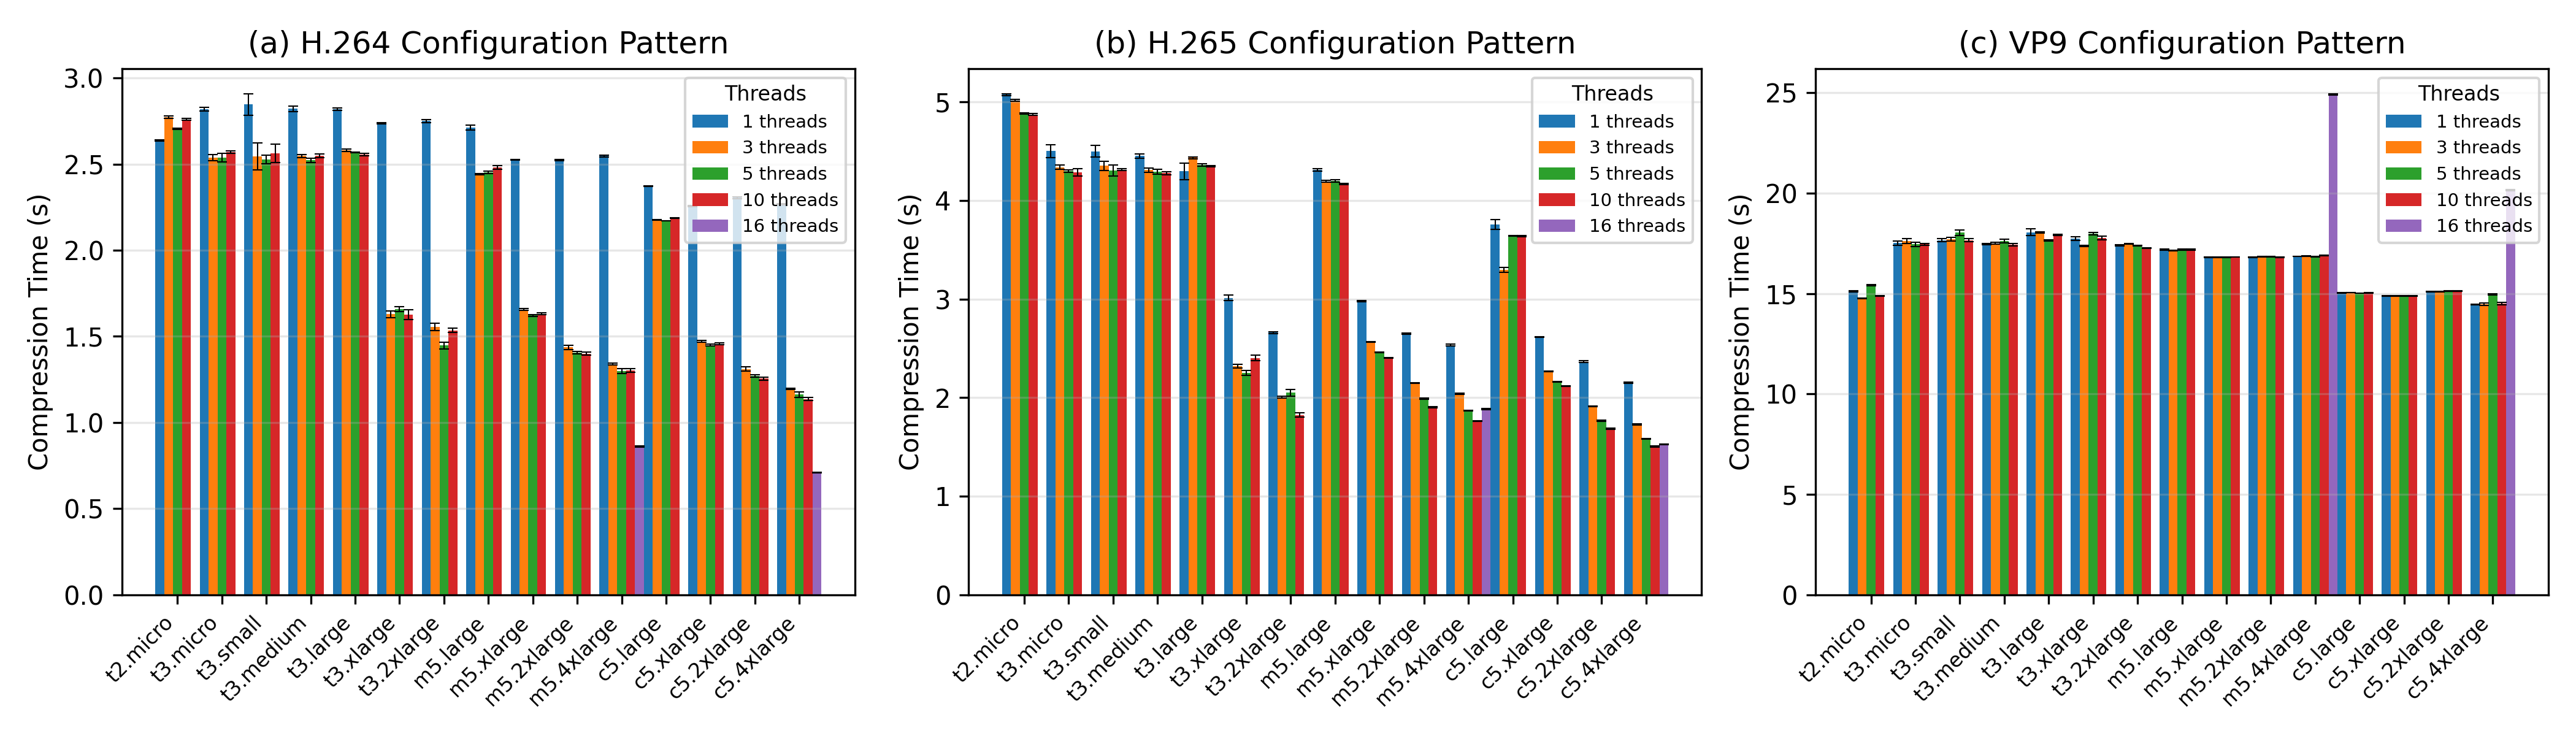
\includegraphics[width=\textwidth]{graphs/unified_codecs_bar_chart.png}
	\caption{Compression time (mean $\pm$ 95\% CI, $n=30$) across all x86 instance
	families for (a) H.264, (b) H.265, and (c) VP9 codecs. C-family instances
	outperform T and M families at equivalent sizes. Thread scaling yields
	diminishing returns beyond 5 threads for H.264 and H.265 on smaller instances,
	while VP9 exhibits near-constant encoding times up to 10 threads, with
	significant regression at 16 threads on larger configurations.}
	\label{fig:unified_codecs}
\end{figure*}

% -----------------------------------------------------------------------
% PHASE 3 RESULTS
% -----------------------------------------------------------------------
\subsection{Phase 3 Results: Horizontal vs. Vertical Scaling Analysis}

Building upon Phase~2 findings that identified \texttt{t3.micro} as the
cost-optimal configuration for H.264 compression, we present a scaling
analysis using a 10-minute video workload. Note that Phase~2 measured raw encoding
time for isolated 30-second segments (median $\approx$2.5\,s for \texttt{t3.micro}),
while Phase~3 measures end-to-end pipeline wall-clock time including provisioning,
file transfer, encoding, and output retrieval. The higher Phase~3 wall-clock values ($\approx$73\,s per
cluster run) reflect the addition of provisioning overhead ($\approx$48\,s), FFmpeg
process startup, and SFTP transfer, which are excluded from Phase~2 measurements. Our Phase~3 evaluation establishes its baseline by isolating the traditional H.264 codec across all x86 architectural families, isolating provisioning dynamics from codec-specific confounds (Table~\ref{tab:scaling_all_families}). Subsequently, rather than re-tabulating the entire x86 grid, we selectively deploy the higher-compression H.265 (HEVC) and VP9 encoders specifically to benchmark the custom ARM Graviton 3 hardware (\texttt{c7g}, \texttt{m7g}) against established x86 performance baselines, revealing codec-specific performance differences across architectures. For the primary H.264 scaling evaluation, our methodology contrasts a cluster of ten
\texttt{t3.micro} instances, each processing one-minute segments in parallel,
against the largest vertical configurations available within each x86 instance
family: \texttt{t3.2xlarge}, \texttt{m5.4xlarge}, and \texttt{c5.4xlarge}. To preserve experimental integrity, we restricted Graviton scaling tests to General Purpose (M) and Compute Optimized (C) instances, excluding burstable T-family variants (e.g., \texttt{t4g}) whose credit-based mechanics introduce noise in sustained benchmarks. The nearest cost-equivalent vertical baseline for the 10-node \texttt{t3.micro}
cluster (\$0.104/h) is the \texttt{t3.xlarge} (\$0.1664/h); however,
benchmarking against the largest nodes of each family (up to \$0.768/h) allows
this study to evaluate whether distributed small-instance clusters outperform
not only their budget-equivalent counterparts, but also the highest-throughput
vertical nodes within each tier.

\subsubsection{Two-Phase Analysis Results}

Phase~3.1 implemented dynamic provisioning with standard Ubuntu images and
post-deployment dependency installation to isolate provisioning overhead from
computational performance, directly quantifying the bottleneck raised in \textbf{RQ2}. This unoptimized baseline, established using the
T-family architecture, revealed that setup activities consumed between 57.3\%
and 93.3\% of total processing time across configurations. Under dynamic
provisioning, vertical scaling (\texttt{t3.2xlarge}) completed the workload in
3.04 minutes, outperforming the horizontal \texttt{t3.micro} cluster (3.28
minutes) by 7.3\%. Despite this performance differential, the horizontal
approach incurred a total cost of \$0.00569 against \$0.01686 for vertical
scaling---a 66.3\% reduction. These results indicate that parallel
orchestration overhead requires mitigation before horizontal scaling can
realize its performance potential, motivating the optimized provisioning
strategy evaluated in Phase~3.2.

Phase~3.2 employed optimized provisioning through custom, pre-configured
Amazon Machine Images (AMIs) that eliminated runtime dependency installation,
mitigating setup overhead across all families and addressing \textbf{RQ3}. The optimized \texttt{t3.micro}
horizontal cluster achieved a total processing time of 1.22 minutes,
representing a $1.48\times$ speedup over the vertical \texttt{t3.2xlarge}
(1.80 minutes). This performance inversion extended to the larger tiers: the
M-family horizontal cluster achieved 1.22 minutes ($1.28\times$ speedup over
the vertical \texttt{m5.4xlarge}, 1.56 minutes), and the C-family cluster
achieved 1.18 minutes ($1.26\times$ speedup over the vertical
\texttt{c5.4xlarge}, 1.49 minutes). The single \texttt{t3.micro} serial
configuration required 2.72 minutes, establishing the non-distributed execution
baseline.

\subsubsection{Analysis and Validation}

In the parallel context, \textit{Effective Encoding Time} encompasses raw FFmpeg
computation plus network I/O transfers (SFTP segment upload and output retrieval),
while \textit{Setup Overhead} denotes the API-to-SSH-ready provisioning latency.
Experimental artifacts are publicly available at \url{https://anonymous.4open.science/r/ec2sweetspot-blinded2}.

Table~\ref{tab:scaling_all_families} presents detailed operational data across
optimization phases, demonstrating that optimized horizontal scaling achieves
improved performance and cost-efficiency.
Figure~\ref{fig:unified_scaling} further illustrates that horizontal scaling
speeds are maximized when provisioning overhead is minimized through AMI
optimization.

\begin{table*}[!htbp]
\centering
\caption{Scaling strategies across optimization phases. \textbf{Prov.}: Dynamic (Ubuntu) vs.\ Optimized (pre-built AMI). \textbf{Speedup} is relative to the serial baseline of each family and provisioning phase. \textbf{Cost$\times$} is total cost relative to the serial AMI baseline. ARM results are in Table~\ref{tab:arm_graviton_scaling}.}
\label{tab:scaling_all_families}
\footnotesize
\begin{tabular}{llcccc}
\toprule
\textbf{Instance} & \textbf{Prov.} & \textbf{Time (min)} & \textbf{Cost (USD)} & \textbf{Speedup} & \textbf{Cost$\times$} \\
\midrule
\multicolumn{6}{c}{\textbf{Burstable T} \quad Serial: \texttt{t3.micro} \quad Parallel: 10$\times$\texttt{t3.micro} \quad Vertical: \texttt{t3.2xlarge}} \\
\midrule
\multirow{2}{*}{\texttt{t3.micro}}      & Dynamic   & 4.03 $\pm$ 0.12 & \$0.00070 & 1.00$\times$ & 1.0$\times$ \\
                                         & Optimized & 2.72 $\pm$ 0.08 & \$0.00047 & 1.00$\times$ & 1.0$\times$ \\
\multirow{2}{*}{10$\times$\texttt{t3.micro}} & Dynamic   & 3.28 $\pm$ 0.10 & \$0.00569 & 1.23$\times$ & 8.1$\times$ \\
                                         & Optimized & 1.22 $\pm$ 0.04 & \$0.00211 & 2.23$\times$ & 4.5$\times$ \\
\multirow{2}{*}{\texttt{t3.2xlarge}}    & Dynamic   & 3.04 $\pm$ 0.09 & \$0.01686 & 1.33$\times$ & 24.1$\times$ \\
                                         & Optimized & 1.80 $\pm$ 0.05 & \$0.00998 & 1.51$\times$ & 21.2$\times$ \\
\midrule
\multicolumn{6}{c}{\textbf{General Purpose M} \quad Serial: \texttt{m5.large} \quad Parallel: 10$\times$\texttt{m5.large} \quad Vertical: \texttt{m5.4xlarge}} \\
\midrule
\multirow{2}{*}{\texttt{m5.large}}      & Dynamic   & 3.46 $\pm$ 0.10 & \$0.00554 & 1.00$\times$ & 1.0$\times$ \\
                                         & Optimized & 2.71 $\pm$ 0.08 & \$0.00434 & 1.00$\times$ & 1.0$\times$ \\
\multirow{2}{*}{10$\times$\texttt{m5.large}} & Dynamic   & 3.63 $\pm$ 0.11 & \$0.05808 & 0.95$\times$ & 10.5$\times$ \\
                                         & Optimized & 1.22 $\pm$ 0.04 & \$0.01952 & 2.22$\times$ & 4.5$\times$ \\
\multirow{2}{*}{\texttt{m5.4xlarge}}    & Dynamic   & 2.33 $\pm$ 0.07 & \$0.02982 & 1.48$\times$ & 5.4$\times$ \\
                                         & Optimized & 1.56 $\pm$ 0.05 & \$0.01997 & 1.74$\times$ & 4.6$\times$ \\
\midrule
\multicolumn{6}{c}{\textbf{Compute Optimized C} \quad Serial: \texttt{c5.large} \quad Parallel: 10$\times$\texttt{c5.large} \quad Vertical: \texttt{c5.4xlarge}} \\
\midrule
\multirow{2}{*}{\texttt{c5.large}}      & Dynamic   & 3.21 $\pm$ 0.10 & \$0.00455 & 1.00$\times$ & 1.0$\times$ \\
                                         & Optimized & 2.46 $\pm$ 0.07 & \$0.00349 & 1.00$\times$ & 1.0$\times$ \\
\multirow{2}{*}{10$\times$\texttt{c5.large}} & Dynamic   & 3.52 $\pm$ 0.11 & \$0.04987 & 0.91$\times$ & 11.0$\times$ \\
                                         & Optimized & 1.18 $\pm$ 0.04 & \$0.01672 & 2.08$\times$ & 4.8$\times$ \\
\multirow{2}{*}{\texttt{c5.4xlarge}}    & Dynamic   & 2.13 $\pm$ 0.06 & \$0.02414 & 1.51$\times$ & 5.3$\times$ \\
                                         & Optimized & 1.49 $\pm$ 0.04 & \$0.01689 & 1.65$\times$ & 4.8$\times$ \\
\bottomrule
\end{tabular}
\end{table*}

The results confirm that the performance advantage of optimized horizontal
scaling holds across all three families. As detailed in
Table~\ref{tab:scaling_all_families}, the M-family horizontal cluster achieved
a $1.28\times$ speedup (1.22 min vs.\ 1.56 min) over the vertical
\texttt{m5.4xlarge}, and the C-family cluster achieved the fastest overall time
of 1.18 minutes ($1.26\times$ speedup vs.\ 1.49 min). The T-family horizontal
cluster (1.22 min) demonstrated the strongest relative speedup at $1.48\times$
over the vertical \texttt{t3.2xlarge} (1.80 min).

These empirical results quantify the cost-performance implications of cloud media scaling strategy selection. As
shown in the Phase~3.2 cost analysis, the optimized horizontal architecture not
only reduced execution time but simultaneously delivered a cost reduction across
all three families relative to their vertical counterparts. The M-family
cluster reduced cost by 2.3\% (\$0.01952 vs.\ \$0.01997) while completing the
workload 21.8\% faster in wall-clock time. The C-family cluster reduced cost by
1.0\% (\$0.01672 vs.\ \$0.01689) while completing the workload 20.8\% faster.
These within-family savings are marginal in absolute terms---the primary
economic advantage of horizontal scaling within the same instance family lies in
the performance gain rather than cost reduction, as the per-hour rates of
smaller instances scale nearly proportionally to those of larger ones.
For cross-family comparisons, the contrast is larger. These comparisons pair burstable T-family instances with general-purpose M-family and compute-optimized C-family instances, which differ in CPU burst behavior and SLA guarantees. The comparison is justified for the specific episodic, short-duration workloads studied here: each \texttt{t3.micro} node processes a 60-second chunk in an ephemeral burst that completes before CPU credits are exhausted---within the burst window, burstable instances deliver sustained 100\% vCPU performance comparable to non-burstable alternatives. Under this burst-compatible workload regime, the \texttt{t3.micro} cluster (\$0.00211) achieved an 89.4\% cost reduction
relative to the \texttt{m5.4xlarge} (\$0.01997) and an 87.5\% cost reduction
relative to the \texttt{c5.4xlarge} (\$0.01689), while outperforming both in
processing speed.

These results demonstrate that vertical scaling is not the only viable approach
for high-performance tasks. Even for Compute Optimized workloads, a cluster of
smaller instances (\texttt{c5.large}) outperformed both the processing speed
and cost of the largest vertical node (\texttt{c5.4xlarge}) when provisioning
overhead was mitigated. The M and C family results empirically demonstrate that
horizontal scaling shifts from an economic compromise to a performance-dominant
strategy for divisible cloud computations.

\begin{figure*}[!ht]
	\centering
	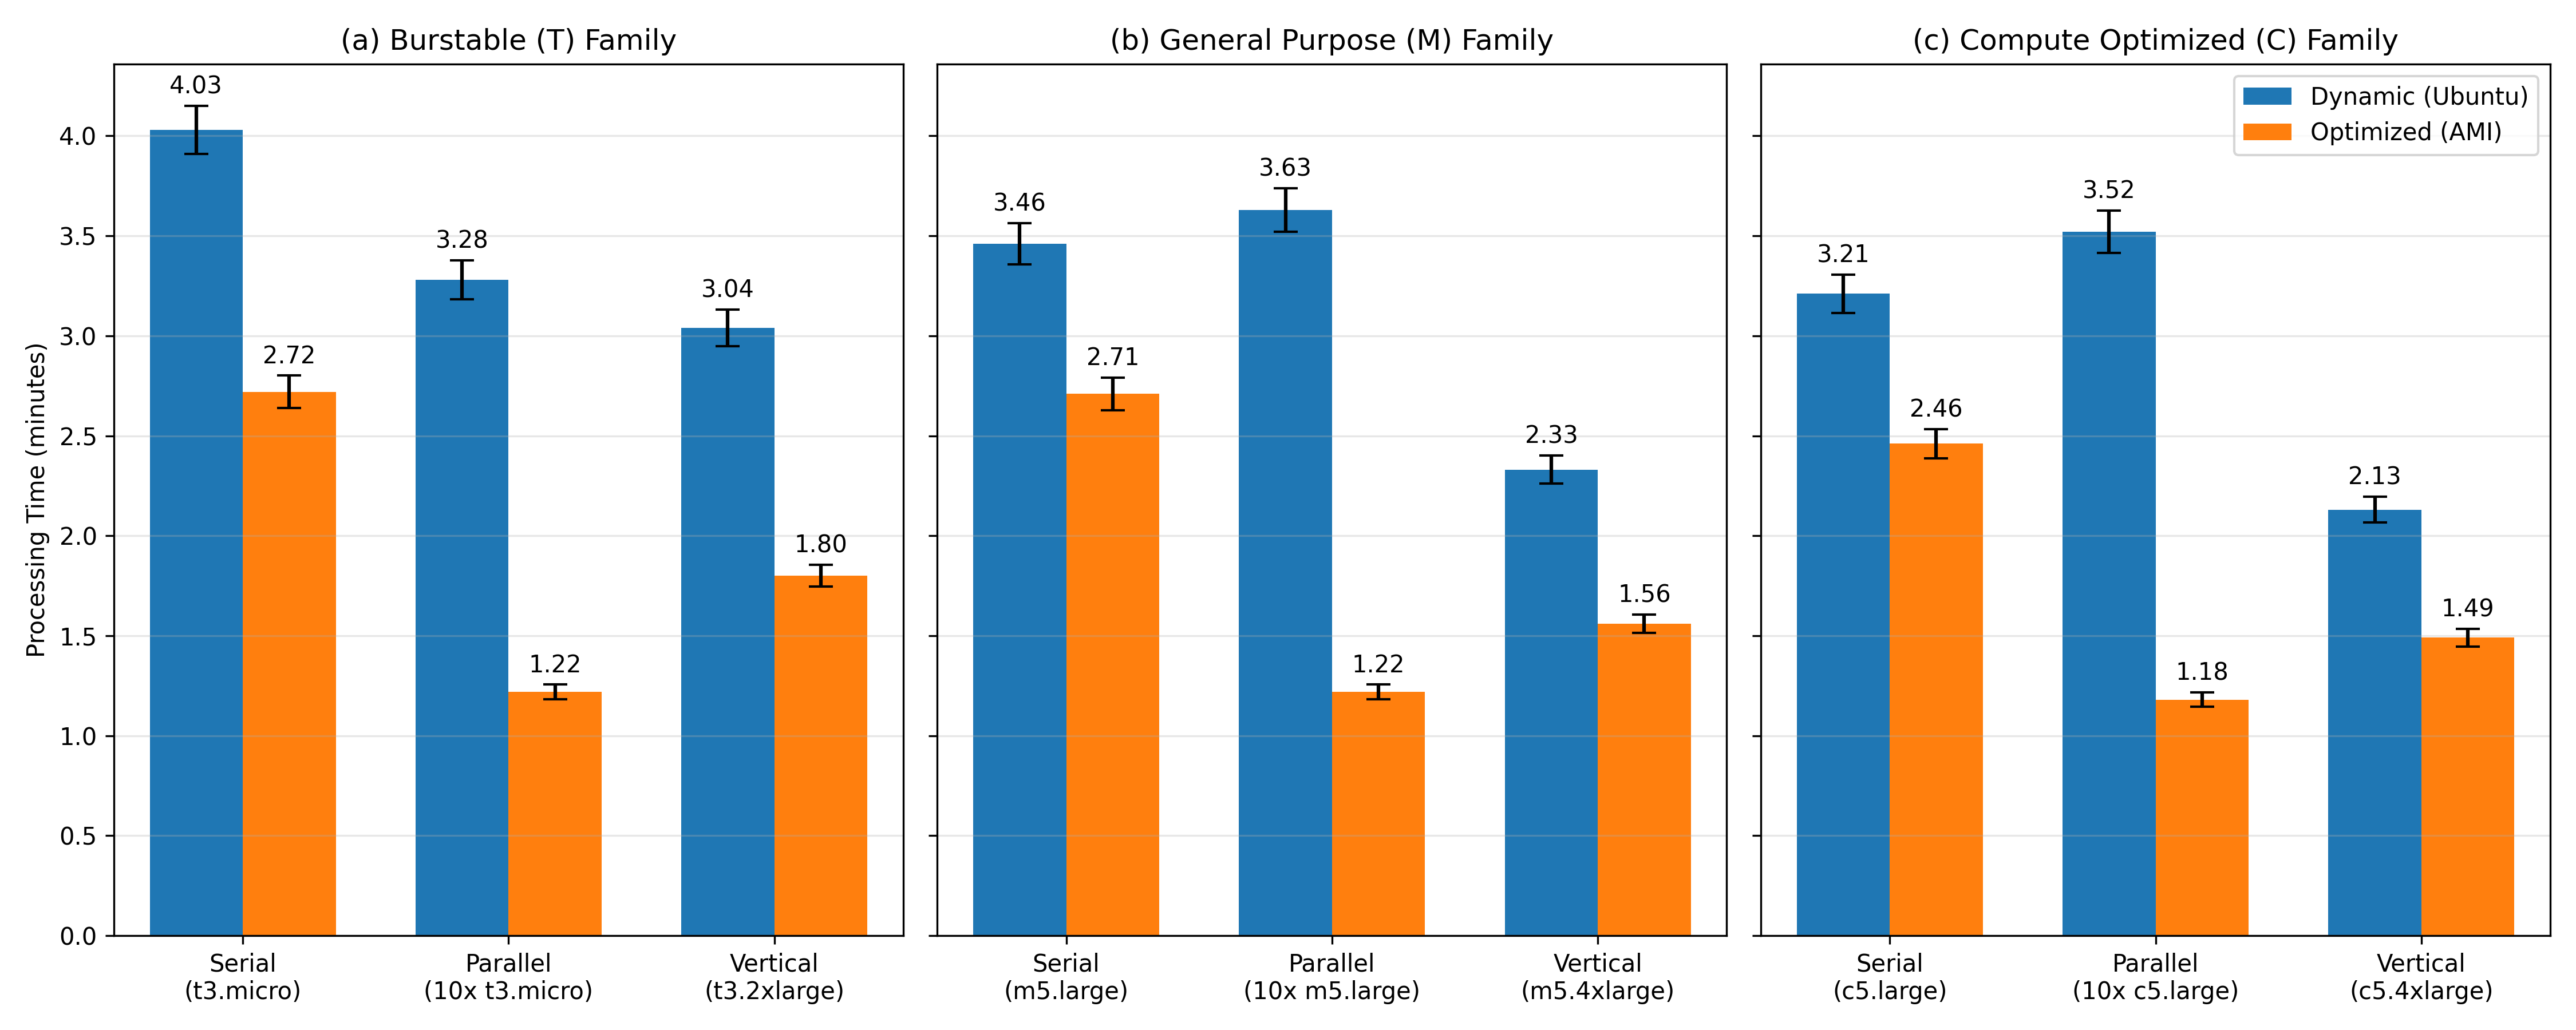
\includegraphics[width=0.7\textwidth]{graphs/unified_scaling_comparison.png}
	\caption{Performance and cost scaling comparison across (a) T, (b) M, and
	(c) C instance families. The composite visualization demonstrates horizontal
	scaling speedup across all configurations when operational provisioning
	overhead is eliminated through pre-compiled AMIs.}
	\label{fig:unified_scaling}
\end{figure*}

\subsubsection{Methodological and Statistical Validation}

The experimental design ensures validation through multiple approaches:
controlled comparison of identical workloads across scaling strategies; direct
quantification of provisioning overhead (57.3\%--93.3\% across T-family Phase~3.1 strategies: serial, parallel, and vertical); and statistical confidence from $n=30$ complete runs
for both Phase~2 micro-benchmarks and Phase~3 macro-architecture configurations.

To validate the Phase~3 horizontal scaling speedups, we applied the same
statistical framework used in Phase~2. Welch's t-tests confirmed statistically
significant speedup advantages for horizontal scaling across all x86 families
($p < 10^{-23}$ for T-family; $p < 10^{-44}$ for M and C families), with large
effect sizes ($d = 3.74$, $d = 8.77$, and $d = 7.69$, respectively). ARM
Graviton configurations, which exhibit higher variance (CV~$>50\%$ for H.265),
are treated as preliminary results and discussed in Section~\ref{limitations}.

These results demonstrate that horizontal scaling's performance advantages can
be realized when operational bottlenecks are addressed. The 78.9\% cost
reduction from the T-family cross-size comparison (10$\times$ \texttt{t3.micro}
vs.\ 1$\times$ \texttt{t3.2xlarge}, Phase~3.2) and the statistically
significant speedup advantages across all tested x86 families together support
systematic re-evaluation of vertical scaling approaches for video encoding
workloads in cloud environments. Unlike the M and C-family comparisons---where
horizontal and vertical configurations are drawn from the same instance tier
range (\texttt{large} vs.\ \texttt{4xlarge})---the T-family result spans the
full burstable size spectrum (micro to 2xlarge), and the magnitude of the cost
advantage reflects this size disparity as much as any architectural benefit of
horizontal scaling.

% -----------------------------------------------------------------------
% EXTENDED EVALUATIONS (M1, M2, M3)
% -----------------------------------------------------------------------
\subsection{Architecture, Codec, and Regional Impact Analysis}

We extended our Phase~3 framework to evaluate the impact of differing CPU architectures, modern codecs, and regional pricing disparities.

\textbf{ARM Graviton Performance (Codecs):} The introduction of ARM Graviton instances (\texttt{c7g.large}, \texttt{m7g.large}) alongside their x86 counterparts revealed architectural sensitivities. While x86 instances exhibited superior performance for traditional H.264 encoding under horizontal scaling (e.g., \texttt{c5.large} achieved a median time of 64.04s in \texttt{us-east-1}), ARM Graviton demonstrated codec-specific parallel encoding advantages for H.265 (HEVC).

Table~\ref{tab:arm_graviton_scaling} details the Phase~3.2 execution results for ARM Graviton processors. The horizontal \texttt{m7g.large} cluster achieved a median of 59.27 seconds for H.265, representing a substantial acceleration over its own serial H.265 baseline (which requires over 11 minutes when encoding the full 10-minute workload serially). Within the ARM architecture, both the \texttt{m7g.large} (59.27s) and \texttt{c7g.large} (61.03s) horizontal clusters achieved comparable H.265 performance, with no statistically significant difference between the two families ($p = .47$). Note that the 59.27s H.265 result should not be directly compared to x86 H.264 horizontal results (e.g., \texttt{c5.large} at 64.04s): these measurements involve different codecs, and such a cross-codec comparison conflates encoder complexity with architectural performance differences.

For the H.264 codec on ARM, serial execution (57.55\,s) outperformed the parallel cluster (108.07\,s)---an inversion attributable to provisioning overhead dominating the $\approx$6\,s per-chunk encoding time on \texttt{m7g.large}.

A notable characteristic of the original \texttt{m7g.large} serial H.265 logs was an apparent outlier: 26 of 27 runs clustered tightly around 700--718\,s (median 700.5\,s), while one run recorded 328.92\,s. Manual inspection revealed that this single low value is a \textit{log-parsing artifact}: the experiment log file contains interleaved output from concurrently executing codec pipelines, and the consolidation script misattributed one VP9 run ($\approx$329\,s, consistent with the VP9 median of 329.03\,s) to the H.265 column. Excluding this artifact, the true H.265 serial distribution for \texttt{m7g.large} is unimodal with very low variance (n=26, median=700.51\,s, stdev=4.10\,s). Table~\ref{tab:arm_graviton_scaling} presents corrected statistics for both H.265 serial rows: \texttt{m7g.large} (n=26) and \texttt{c7g.large} (n=29, one misattributed run similarly excluded).

\begin{table*}[h]
	\centering
	\caption{Descriptive statistics for compression time (seconds), efficiency, and total cost for ARM Graviton configurations. $^{\dagger}$H.265 serial statistics corrected after removing log-parsing artifact: m7g.large n=26 (1 misattributed VP9 run excluded); c7g.large n=29 (1 misattributed H.264 run excluded). $^{\ddagger}$\texttt{m7g.large} horizontal H.264: n=24 (resumed after early session crash; 6 preliminary runs excluded from final aggregate). All other rows use n=30.}
	\label{tab:arm_graviton_scaling}
	\small
	\resizebox{\textwidth}{!}{%
		\begin{tabular}{ll|rrrrr|rrrrr|rrrrr}
			\toprule
			& & \multicolumn{5}{c|}{H.264} & \multicolumn{5}{c|}{H.265 (libx265)} & \multicolumn{5}{c}{VP9 (libvpx-vp9)} \\
			\cmidrule(lr){3-7} \cmidrule(lr){8-12} \cmidrule(lr){13-17}
			& & \multicolumn{4}{c}{Compression Time (s)} & \multicolumn{1}{c|}{Eff. | Cost (\$)} & \multicolumn{4}{c}{Time (s)} & \multicolumn{1}{c|}{Eff. | Cost (\$)} & \multicolumn{4}{c}{Time (s)} & \multicolumn{1}{c}{Eff. | Cost (\$)} \\
			Instance Type & Strategy & Median & Std & Min & Max & (Median) & Median & Std & Min & Max & (Median) & Median & Std & Min & Max & (Median) \\
			\midrule
			m7g.large & serial & \textbf{57.5500} & 0.6145 & 57.3800 & 60.1400 & \textbf{13} | \textbf{0.0013045} & 700.5100$^{\dagger}$ & 4.0974 & 699.8900 & 718.5100 & 0 | 0.0158782 & 329.0300 & 1.4109 & 327.6800 & 333.0200 & 0 | 0.0074580 \\
			m7g.large & horizontal & 108.0700$^{\ddagger}$ & 16.6122 & 60.9900 & 150.0600 & 3 | 0.0024496 & \textbf{59.2650} & 30.5831 & 58.0900 & 225.7900 & \textbf{12} | \textbf{0.0013433} & 105.2050 & 27.3938 & 59.0200 & 134.8600 & 3 | 0.0023846 \\
			\cmidrule(lr){1-17}
			c7g.large & serial & \textbf{58.1700} & 32.2485 & 57.0300 & 151.6700 & \textbf{14} | \textbf{0.0011699} & 702.1500$^{\dagger}$ & 1.3618 & 701.6200 & 709.3800 & 0 | 0.0141405 & 328.7450 & 1.5953 & 327.3100 & 336.4100 & 0 | 0.0066114 \\
			c7g.large & horizontal & 107.6800 & 18.3406 & 60.9700 & 171.0600 & 4 | 0.0021656 & \textbf{61.0300} & 2.7580 & 58.4100 & 72.4300 & \textbf{13} | \textbf{0.0012274} & \textbf{70.6100} & 30.3532 & 57.9700 & 191.4100 & \textbf{9} | \textbf{0.0014200} \\
			\bottomrule
		\end{tabular}%
	}
\end{table*}

\textbf{Statistical Validation of Novel Architectures:} Non-parametric testing (Mann-Whitney~U, $p > .05$) revealed no statistically significant performance difference between \texttt{m7g.large} and \texttt{c7g.large} for H.265 horizontal encoding, though the high coefficient of variation (CV~$>50\%$) limits statistical power. Welch's t-test confirmed the H.264 performance inversion on \texttt{m7g.large} ($p < 10^{-12}$, Cohen's $d = 4.31$): provisioning overhead dominates encoding time, rendering horizontal scaling inviable for \texttt{libx264} on Graviton under the evaluated conditions.

\textbf{Regional Cost Disparities:} Replication in \texttt{sa-east-1} (São Paulo) reveals a price differential of 54--62\% over \texttt{us-east-1}, varying by family (T: 61.5\%, M: 59.4\%, C: 54.1\%). For the H.264 horizontal strategy (10$\times$ nodes, 60\,s chunks), cluster costs roughly double: \texttt{t3.micro} \$0.0021 vs.\ \$0.0045; \texttt{m5.large} \$0.0150 vs.\ \$0.0339; \texttt{c5.large} \$0.0152 vs.\ \$0.0234. Wall-clock times remain comparable across regions, confirming that compute performance is architecture-bound rather than region-bound.

\subsection{Phase 4 Results: Chunk Size Sensitivity and Cost Analysis}
\label{results-phase4}

Phase 4 extends the empirical observations from the preceding phases with a sensitivity analysis of chunk duration and a cost model for pipeline economics, addressing \textbf{RQ4} on regional pricing and network egress constraints.

\textbf{Empirical Chunk Size Sensitivity:}
The speedup of a horizontally scaled transcoding cluster is bound by the intersection of parallelization efficiency and orchestration overhead. Let $S(c)$ represent the speedup factor as a function of chunk duration $c$. The total execution time $T(c)$ for a video of length $L$ across $N = \lceil L/c \rceil$ instances is modeled as:
\begin{equation}
T(c) = t_{\text{seg}} + \max_{1 \le i \le N} \left( t_{\text{prov},i} \right) + t_{\text{enc}}(c) + t_{\text{merge}}
\end{equation}
where $t_{\text{prov},i}$ represents the provisioning and boot latency of the $i$-th instance, and $t_{\text{enc}}(c)$ is the encoding duration for a chunk of length $c$. As $c$ decreases, $N$ increases, monotonically elevating the probability of a high $t_{\text{prov},i}$ long-tail outlier bound (the synchronization barrier). To empirically quantify this sensitivity, we evaluated the 10-minute H.264 workload with 30-second ($N=20$), 60-second ($N=10$), and 120-second ($N=5$) chunks. Total Time is measured end-to-end, comprising video segmentation, parallel AWS provisioning (\texttt{boto3} waiter + 30\,s SSH readiness wait per instance), segment transfer, encoding, and output retrieval. Results are presented in Table~\ref{tab:chunk_sensitivity}.

The findings confirm a sensitivity trade-off: 30-second chunks increase coordination overhead (20 bootstrap sequences instead of 10), reducing speedup; 120-second chunks reduce provisioning calls but fail to achieve sufficient parallelism. The 60-second configuration achieves the optimal balance, yielding the highest speedup across all families (1.48$\times$ for T, 1.28$\times$ for M, and 1.26$\times$ for C).

\begin{table}[h]
	\centering
	\caption{Chunk Size Sensitivity Analysis (10-min H.264, Phase 3.2 AMI).
	Total Time is end-to-end wall-clock. Speedup vs.\ the single-instance vertical baseline of each family (\texttt{t3.2xlarge}: 1.81\,min; \texttt{m5.4xlarge}: 1.56\,min; \texttt{c5.4xlarge}: 1.49\,min).}
	\label{tab:chunk_sensitivity}
	\resizebox{\columnwidth}{!}{
		\begin{tabular}{|l|l|c|c|}
			\hline
			\textbf{Family} & \textbf{Chunk Strategy} & \textbf{Total Time (min)} & \textbf{Speedup vs Vertical} \\
			\hline
			\multirow{3}{*}{Burstable (T)} & 30s (20x t3.micro) & 1.39 & 1.30$\times$ \\
			& \textbf{60s (10x t3.micro)} & \textbf{1.22} & \textbf{1.48$\times$} \\
			& 120s (5x t3.micro) & 2.04 & 0.88$\times$$^{*}$ \\
			\hline
			\multirow{3}{*}{General (M)} & 30s (20x m5.large) & 1.63 & 0.96$\times$$^{*}$ \\
			& \textbf{60s (10x m5.large)} & \textbf{1.22} & \textbf{1.28$\times$} \\
			& 120s (5x m5.large) & 2.10 & 0.74$\times$$^{*}$ \\
			\hline
			\multirow{3}{*}{Compute (C)} & 30s (20x c5.large) & 1.44 & 1.03$\times$ \\
			& \textbf{60s (10x c5.large)} & \textbf{1.18} & \textbf{1.26$\times$} \\
			& 120s (5x c5.large) & 1.98 & 0.75$\times$$^{*}$ \\
			\hline
			\multicolumn{4}{|l|}{\footnotesize $^{*}$ Speedup $< 1.0\times$ indicates horizontal cluster is \textit{slower} than vertical.} \\
			\hline
		\end{tabular}
	}
\end{table}

\textbf{The Network Egress Economic Bottleneck:}
While optimized chunking minimizes compute expenditure, full cloud pipeline economics demand a deterministic cost model. Total Cost ($C_{\text{total}}$) is formulated as the sum of compute provisioning ($C_{\text{comp}}$) and outbound data transfer ($C_{\text{net}}$) (Eq.~\ref{eq:cost_model}):
\begin{equation}
\label{eq:cost_model}
C_{\text{total}} = \left( \sum_{i=1}^{N} R_{\text{inst}} \times T_{i} \right) + \left( R_{\text{egress}} \times D_{\text{out}} \right)
\end{equation}
where $R_{\text{inst}}$ is the per-second instance billing rate, $T_i$ is the active billing lifespan of node $i$,\footnote{AWS imposes a 60-second minimum billing floor per instance: any $T_i < 60$\,s is billed as 60\,s. All $T_i$ values observed in our experiments exceed this threshold.} $R_{\text{egress}}$ is the regional outbound internet data transfer rate (e.g., \$0.09/GB in \texttt{us-east-1}, \$0.25/GB in \texttt{sa-east-1}), and $D_{\text{out}}$ is the final payload size in GB.

Our network analysis indicates that intra-region transfers incur no additional per-GB charges. Outbound internet egress, however, imposes a fixed economic floor: delivering the $\approx$100\,MB H.264 output incurs $\approx$\$0.009 in \texttt{us-east-1} ($\approx$4$\times$ the optimized \texttt{t3.micro} compute cost of \$0.00211), making egress the dominant cost component once compute is optimized.

% -----------------------------------------------------------------------
% DISCUSSION AND THREATS TO VALIDITY
% -----------------------------------------------------------------------
\section{Discussion and Threats to Validity}
\label{limitations}

While our findings advocate for optimized horizontal scaling, several operational constraints and validity threats must be acknowledged when generalizing these results.

\textbf{Docker Container vs.\ AMI Overhead:} In Phase~3.2, the custom AMI pre-installs FFmpeg and all dependencies; no Docker layer pull occurs at runtime. The observed provisioning overhead ($\approx$48\,s) reflects EC2 instance launch time, EBS volume attachment, OS boot, and SSH readiness---not container registry download. In Phase~3.1, FFmpeg is installed post-boot via \texttt{apt}, accounting for the higher setup times in that phase.

\textbf{Burstable Instance CPU Credits:} T-family instances operate in Unlimited mode~\cite{awscredits}, consuming Surplus Credits immediately upon launch. In the ephemeral orchestration pattern used here (spawn, encode, terminate), instances do not accumulate idle time to repay credit deficits. Two bounds characterize the surcharge exposure: under a realistic encoding-focused estimate ($\approx$22\,s at full CPU), the per-cluster surcharge is $\approx$\$0.0055, raising the cluster cost to $\approx$\$0.0076 ($\approx$62\% below \texttt{m5.4xlarge}); under the worst case (100\% CPU for the full 73\,s), the surcharge is $\approx$\$0.0183, raising the cluster cost to $\approx$\$0.0204 and eliminating the cost advantage. Billing statements were not audited; the true value lies between these bounds.

\textbf{Serverless and Managed Service Alternatives:} This study evaluates on-demand EC2 instances with custom orchestration. AWS-native managed services (e.g., AWS Elemental MediaConvert, AWS Fargate) offer near-zero provisioning overhead by design; a direct comparison against these alternatives is an important direction for future work.

\textbf{Spot Instance Comparison:} On-demand pricing was used throughout to ensure deterministic completion. Spot instances represent a materially cheaper alternative documented in related work~\cite{b21,b19}, but introduce preemption risk; this comparison is left for future evaluation.

\textbf{Network Conditions and Transfer Overhead:} All experiments were conducted within a single AWS availability zone, with SFTP transfers between the orchestrating host and worker nodes. AZ-internal network bandwidth and SFTP throughput were not independently characterized; uncontrolled variability in the transfer phase is conflated with encoding time in wall-clock measurements, limiting the interpretability of timing decompositions.

\textbf{Workload Representativeness:} The sensitivity analysis was conducted on a single 10-minute, 720p video. The optimal 60-second chunk duration may not generalize across different video lengths, resolutions, or complexity profiles, and should be treated as a starting point for workload-specific calibration.

\textbf{ARM Graviton Homogeneity Scope:} The 100\% processor homogeneity observed for ARM Graviton instances was validated exclusively within \texttt{us-east-1}. AWS's silicon deployment policy may differ in other regions; the homogeneity claim should not be assumed to hold universally without independent validation.

\textbf{Co-tenancy:} All experiments used shared-tenancy on-demand instances, subject to noisy neighbor variability. The 30-iteration design and low coefficient of variation ($<$0.6\% for Phase~2 benchmarks) suggest co-tenancy effects were minimal during measurement windows, but cannot be fully excluded without dedicated-tenancy replication.

\textbf{Generalizability:} Experiments were constrained to \texttt{us-east-1}, x86 architectures, and three standard codecs, with ARM Graviton and \texttt{sa-east-1} validation included. Absolute economic claims must be contextualized: AWS pricing and hardware generations evolve continuously, and the identified configurations reflect conditions at the time of experimentation. Extension to GPU-accelerated instances and custom-compiled ARM-native encoder binaries are important directions for future work.

% -----------------------------------------------------------------------
% CONCLUSION
% -----------------------------------------------------------------------
\section{Conclusion}
\label{conclusion}

This study demonstrates that, in the evaluated horizontal scaling configurations for short-form video encoding, operational provisioning overhead accounts for the largest share of total processing time---up to 93.3\% in unoptimized T-family deployments (Phase~3.1)---rather than raw hardware throughput.

By implementing an optimized custom AMI orchestration framework, we eliminated this setup latency. In fully optimized parallel environments, distributed clusters of small instances (e.g., 10$\times$ \texttt{t3.micro}) outperformed single maximal instances (e.g., \texttt{c5.4xlarge}) across all evaluated families under 60-second chunk partitioning, achieving an 89.4\% base-compute cost reduction relative to \texttt{m5.4xlarge} while simultaneously accelerating task completion.

Our analysis revealed codec-specific architectural sensitivities: ARM Graviton horizontal clusters achieved competitive H.265 performance (median 59.27\,s on \texttt{m7g.large}), though with high execution time variability (CV~$>50\%$). Chunk size sensitivity analysis identified 60-second partitioning as optimal across all three x86 families. Network cost analysis confirmed that outbound internet egress emerges as the primary economic bottleneck once compute provisioning is optimized.

Future research should extend this methodology to GPU-accelerated instances and evaluate spot instance pricing as an alternative cost baseline. This work establishes an empirical foundation for cloud media processing, demonstrating that provisioning latency mitigation is a prerequisite to realizing the cost-performance potential of horizontally scaled cloud architectures.

% APPENDIX removed — submitted as separate document
% -----------------------------------------------------------------------
%\appendices
%\section{Artifact Documentation: EC2 Sweet Spot}
%\label{app:artifact}

%This appendix documents the research artifacts for the ``EC2 Sweet Spot'' study
%on Amazon EC2 instance selection for video compression workloads. All
%experimental materials are available at
%\url{https://anonymous.4open.science/r/ec2sweetspot-blinded2}.
%
%\subsection{Artifact Overview}
%
%The artifact collection contains:
%\begin{itemize}
%	\item Complete experimental setup and configuration files
%	\item Raw and processed performance data from over 4,100 instance deployments
%	\item Benchmarking scripts for performance evaluation
%	\item Data processing pipelines for statistical analysis
%	\item Reproduction scripts for all experimental phases
%\end{itemize}
%
%\subsection{Experimental Methodology}
%
%The artifact supports four experimental phases:
%
%\textbf{Phase 1: Hardware Homogeneity Validation}
%\begin{itemize}
%	\item CPU model verification across 6 AWS availability zones
%	\item Analysis of processor distribution patterns
%	\item Automatic retry mechanisms for hardware validation
%\end{itemize}
%
%\textbf{Phase 2: Performance Benchmarking}
%\begin{itemize}
%	\item Evaluation of 15 EC2 instance types (7 T-family including t2.micro, 4 M-family, 4 C-family)
%	\item Three video codecs (H.264, H.265, VP9) with 4 thread configurations
%	\item 30 iterations per configuration for statistical significance
%	\item Cost-efficiency calculations based on AWS pricing
%\end{itemize}
%
%\textbf{Phase 3: Scaling Strategy Analysis}
%\begin{itemize}
%	\item Comparison of horizontal vs.\ vertical scaling approaches
%	\item Dynamic provisioning vs.\ optimized AMI deployment
%	\item Complete workflow timing and cost analysis
%\end{itemize}
%
%\subsection{Data Collection}
%
%The artifact includes:
%\begin{itemize}
%	\item Over 4,100 CPU verification logs from \texttt{/proc/cpuinfo}
%	\item Over 60 structured execution logs with detailed timing information
%	\item 9 CSV files with aggregated performance metrics
%	\item Raw timing data for over 6,500 benchmark executions (Phase~2: $15 \times 4 \times 3 \times 30 = 5{,}400$; Phase~3 x86 scaling: $\approx$540; ARM Graviton: $\approx$240; Phase~4 chunk sensitivity: $\approx$270; sa-east-1 regional: 90)
%\end{itemize}
%
%\subsection{Reproduction Requirements}
%
%\textbf{Infrastructure:}
%\begin{itemize}
%	\item AWS EC2 access in \texttt{us-east-1} and \texttt{sa-east-1} regions
%	\item Support for 17 EC2 instance types: 15 x86 (7 T-family including t2.micro, 4 M-family, 4 C-family) and 2 ARM Graviton 3 (m7g.large, c7g.large)
%	\item Ubuntu 22.04 LTS base AMI (\texttt{us-east-1}: ami-0a313d6098716f372; AMI IDs are region-specific---for \texttt{sa-east-1} and ARM configurations, use the equivalent Ubuntu 22.04 LTS AMI for that region, available via AWS EC2 AMI catalog)
%	\item Custom AMI with pre-installed dependencies (\texttt{us-east-1}: ami-0300cfb109571fb0b; equivalent AMIs must be built for other regions using the provided Packer/setup scripts in the artifact repository)
%\end{itemize}
%
%\textbf{Software Dependencies:}
%\begin{itemize}
%	\item Python 3.8+ with boto3, paramiko, pandas, numpy, matplotlib
%	\item Docker for containerized FFmpeg execution
%	\item AWS CLI with appropriate EC2 permissions
%\end{itemize}
%
%\textbf{Estimated Reproduction Cost:} \$400--\$600 (AWS instance hours, breakdown: Phase~2 benchmarks $\approx$\$50--\$80; Phase~3 x86 scaling $\approx$\$100--\$150; ARM Graviton evaluation $\approx$\$80--\$120; sa-east-1 regional replication $\approx$\$60--\$100; Phase~4 chunk sensitivity $\approx$\$40--\$60; data transfer and miscellaneous $\approx$\$30--\$60). Note: costs scale with AWS pricing at time of reproduction and may vary by region.\\
%\textbf{Estimated Time:} 4--6 days for complete reproduction
%
%\subsection{Artifact Structure}
%
%The repository contains the following components:
%\begin{itemize}
%	\item \texttt{experimental\_data/} --- Processed results in CSV format
%	\item \texttt{phase1\_homogeneity/} --- CPU validation data and analysis
%	\item \texttt{phase2\_benchmarks/} --- Performance benchmarking scripts
%	\item \texttt{phase3\_scaling/} --- Scaling strategy analysis scripts
%	\item \texttt{scripts/processing/} --- Data analysis pipelines
%	\item \texttt{test\_videos/} --- Benchmark media files (20\,MB, 51\,MB, 2.5\,MB)
%	\item \texttt{documentation/} --- Reproduction guides and validation
%\end{itemize}
%
%\subsection{Extended Evaluations}
%
%The artifact repository also documents two extended experiments conducted beyond the core x86 Phase~3 scaling analysis:
%
%\textbf{ARM Graviton Extended Evaluation:} Scripts and raw data for the \texttt{m7g.large} and \texttt{c7g.large} experiments (H.264, H.265, and VP9 codecs, serial and horizontal strategies) are located in \texttt{phase3\_scaling/arm\_graviton/}. The ARM AMI configuration and CPU verification scripts are documented in \texttt{phase3\_scaling/arm\_setup.md}. Note that ARM AMI IDs differ from x86 IDs and must be resolved separately for each target region.
%
%\textbf{Regional Pricing Evaluation (\texttt{sa-east-1}):} Scripts and processed results for the São Paulo region replication (H.264 horizontal, \texttt{t3.micro}, \texttt{m5.large}, \texttt{c5.large}) are in \texttt{phase3\_scaling/sa\_east\_1/}. The 44\% regional price premium is captured in the experimental configuration files under \texttt{experimental\_data/regional/}.
%
%\subsection{Validation}
%
%All experimental results in the main paper can be reproduced using the artifact
%repository at \url{https://anonymous.4open.science/r/ec2sweetspot-blinded2}, the
%reproduction scripts in \texttt{scripts/processing/}, and the validation
%procedures documented in \texttt{CHECKLIST.md}. The artifact provides complete
%methodological transparency and enables independent verification of all findings
%presented in this work.
%
% -----------------------------------------------------------------------
% BIBLIOGRAPHY
% -----------------------------------------------------------------------
\begin{thebibliography}{00}

\bibitem{b1} W. Maas, F. Rossi, M. Caggiani, P. Navaux, and A. Lorenzon,
``Investigating cloud instances to achieve optimal trade-offs between
performance-cost efficiency,'' \emph{Computing}, vol. 107, no. 1,
pp. 82--97, Jan. 2025. doi: 10.1007/s00607-025-01444-9.

\bibitem{b2} P. Álvarez, S. Hernández, J. Fabra, and J. Ezpeleta,
``Cost-driven provisioning and execution of a computing-intensive service on
the Amazon EC2,'' \emph{The Computer Journal}, vol. 61, no. 9,
pp. 1407--1421, Jan. 2018. doi: 10.1093/comjnl/bxy006.

\bibitem{b3} T. Dancheva, U. Alonso, and M. D. Barton, ``Cloud benchmarking
and performance analysis of an HPC application in Amazon EC2,''
\emph{Cluster Computing}, vol. 27, no. 2, pp. 2273--2290, Jun. 2023.
doi: 10.1007/s10586-023-04060-4.

\bibitem{b4} L. M. Haji, S. R. M. Zeebaree, O. M. Ahmed, A. B. Sallow,
K. Jacksi, and R. R. Zeabri, ``Dynamic Resource Allocation for Distributed
Systems and Cloud Computing,'' \emph{Test Engineering and Management},
vol. 83, no. 1, pp. 22417--22426, Jun. 2020.

\bibitem{b5} Z. Ou, H. Zhuang, J. K. Nurminen, A. Ylä-Jääski, and P. Hui,
``Exploiting Hardware Heterogeneity within the Same Instance Type of Amazon
EC2,'' in \emph{Proc. 4th USENIX Conf. Hot Topics Cloud Comput.}, Boston,
MA, USA, 2012, pp. 4--4.

\bibitem{b6} Z. Ou, H. Zhuang, A. Lukyanenko, J. K. Nurminen, P. Hui,
V. V. Mazalov, and A. Ylä-Jääski, ``Is the Same Instance Type Created Equal?
Exploiting Heterogeneity of Public Clouds,'' \emph{IEEE Trans. Cloud Comput.},
vol. 1, no. 2, pp. 201--214, Jan. 2013. doi: 10.1109/TCC.2013.12.

\bibitem{b7} B. Farley, A. Juels, V. Varadarajan, T. Ristenpart, K. D. Bowers,
and M. M. Swift, ``More for Your Money: Exploiting Performance Heterogeneity
in Public Clouds,'' in \emph{Proc. 3rd ACM Symp. Cloud Comput.}, San Jose,
CA, USA, 2012, pp. 20:1--20:14. doi: 10.1145/2391229.2391249.

\bibitem{b8} A. Katsenou, X. Wang, D. Schien, and D. Bull, ``Comparative Study
of Hardware and Software Power Measurements in Video Compression,'' in
\emph{2024 Picture Coding Symp. (PCS)}, Taichung, Taiwan, 2024, pp. 1--5.
doi: 10.1109/PCS60826.2024.10566286.

\bibitem{b9} A. Pereira Ferreira and R. O. Sinnott, ``A Performance Evaluation
of Containers Running on Managed Kubernetes Services,'' in \emph{2019 IEEE
Int. Conf. Cloud Comput. Technol. Sci. (CloudCom)}, Sydney, Australia, 2019,
pp. 199--208. doi: 10.1109/CloudCom.2019.00038.

\bibitem{b10} J. Scheuner and P. Leitner, ``Estimating Cloud Application
Performance Based on Micro-Benchmark Profiling,'' in \emph{2018 IEEE 11th
Int. Conf. Cloud Comput. (CLOUD)}, San Francisco, CA, USA, 2018, pp. 90--97.
doi: 10.1109/CLOUD.2018.00019.

\bibitem{b11} S. Ebneyousef and S. Ghazanfari-Rad, ``Cloud Resource Demand
Prediction to Achieve Efficient Resource Provisioning,'' in \emph{2022 8th
Iranian Conf. Signal Process. Intell. Syst. (ICSPIS)}, Tehran, Iran, 2022,
pp. 1--6. doi: 10.1109/ICSPIS56952.2022.10043900.

\bibitem{b12} T. S. Nikoui, A. Balador, A. M. Rahmani, and Z. Bakhshi,
``Cost-Aware Task Scheduling in Fog-Cloud Environment,'' in \emph{2020
CSI/CPSSI Int. Symp. Real-Time Embedded Syst. Technol. (RTEST)}, Tehran,
Iran, 2020, pp. 1--8. doi: 10.1109/RTEST49666.2020.9140118.

\bibitem{b13} Y. Yang and H. Casanova, ``RUMR: Robust Scheduling for Divisible
Workloads,'' in \emph{Proc. 12th IEEE Int. Symp. High Perform. Distrib.
Comput.}, Seattle, WA, USA, 2003, pp. 114--123.
doi: 10.1109/HPDC.2003.1210021.

\bibitem{b14} J. Praveenchandar and A. Tamilarasi, ``Resource Allocation Using
Phase Change Hyper Switching Algorithm in the Cloud Environment,''
\emph{Intell. Autom. Soft Comput.}, vol. 34, no. 3, pp. 1839--1850,
Aug. 2022. doi: 10.32604/iasc.2022.026354.

\bibitem{b15} R. Rosado, O. Santos, F. Oliveira, L. Silva, G. Sanchez,
I. Storch, D. Palomino, and L. Agostini, ``A Coding-Efficiency-Aware Fast
Heuristic for VVC Intra-Frame Prediction Targeting 360° Videos,'' in
\emph{Proc. 30th Brazilian Symp. Multimedia Web}, Juiz de Fora, Brazil, 2024,
pp. 355--359. doi: 10.5753/webmedia.2024.243128.

\bibitem{b16} L. Araújo, A. Duarte, G. Correa, B. Zatt, and D. Palomino,
``Fast ISP Mode Decision for the Versatile Video Coding Intra Prediction Using
Machine Learning,'' in \emph{Proc. 30th Brazilian Symp. Multimedia Web},
Juiz de Fora, Brazil, 2024, pp. 162--170. doi: 10.5753/webmedia.2024.243129.

\bibitem{b17} A. Mahida, ``Comprehensive Review on Optimizing Resource
Allocation in Cloud Computing for Cost Efficiency,'' \emph{J. Artif. Intell.
Cloud Comput.}, vol. 1, no. 2, pp. 1--4, May 2022.
doi: 10.47363/JAICC/2022(1)232.

\bibitem{b18} O. Alzakholi, L. M. Haji, H. M. Shukur, R. R. Zebari,
S. M. Abas, and M. Sadeeq, ``Comparison Among Cloud Technologies and Cloud
Performance,'' \emph{J. Appl. Sci. Technol. Trends}, vol. 1, no. 1,
pp. 40--47, Apr. 2020. doi: \url{https://doi.org/10.38094/jastt1219}.

\bibitem{b19} O. A. Ben-Yehuda, M. Ben-Yehuda, A. Schuster, and D. Tsafrir,
``Deconstructing Amazon EC2 Spot Instance Pricing,''
\emph{ACM Trans. Econ. Comput.}, vol.\ 1, no.\ 3, pp.\ 16:1--16:20, Sep.\ 2013.
doi: 10.1145/2509413.2509416.

\bibitem{b20} F. Jiang, K. Ferriter, and C. Castillo, ``A Cloud-Agnostic
Framework to Enable Cost-Aware Scheduling of Applications in a Multi-Cloud
Environment,'' in \emph{2020 IEEE/IFIP Network Operations and Management
Symposium (NOMS)}, Budapest, Hungary, 2020, pp. 1--9.
doi: 10.1109/NOMS47738.2020.9110325.

\bibitem{b21} A. Zabrovskiy, P. Agrawal, V. Kashansky, R. Kersche,
C. Timmerer, and R. Prodan, ``FSpot: Fast and Efficient Video Encoding
Workloads Over Amazon Spot Instances,'' \emph{Computers, Materials \&
Continua}, vol. 71, no. 3, pp. 5677--5694, 2022.
doi: 10.32604/cmc.2022.023630.

\bibitem{b22} W. Moina-Rivera, M. Garcia-Pineda, J. Gutiérrez-Aguado, and
J. M. Alcaraz-Calero, ``Cloud media video encoding: review and challenges,''
\emph{Multimedia Tools and Applications}, vol. 83, pp. 81231--81278, 2024.
doi: 10.1007/s11042-024-18763-2.

\bibitem{b23} W. Maas, F. D. Rossi, M. C. Luizelli, P. O. A. Navaux, and
A. F. Lorenzon, ``Towards Optimizing Cost and Performance for Parallel
Workloads in Cloud Computing,'' in \emph{Proc. 15th Int. Conf. Cloud Comput.
and Services Science (CLOSER)}, 2025, pp. 231--238.
doi: \url{https://doi.org/10.5220/0013421600003950}.


\bibitem{awscredits} Amazon Web Services, ``Burstable performance instances,''
\emph{Amazon EC2 User Guide}, 2024. [Online]. Available:
\url{https://docs.aws.amazon.com/AWSEC2/latest/UserGuide/burstable-performance-instances.html}
[Accessed: Mar.\ 2026].

\bibitem{dockercoldstart} W. Felter, A. Ferreira, R. Rajamony, and J. Rubio,
``An Updated Performance Comparison of Virtual Machines and Linux Containers,''
in \emph{2015 IEEE Int. Symp. Perform. Anal. Syst. Softw. (ISPASS)},
Philadelphia, PA, USA, 2015, pp. 171--172.
doi: 10.1109/ISPASS.2015.7095802.

\bibitem{awsgrav3} Amazon Web Services, ``AWS Graviton3 Processor,''
\emph{Amazon EC2 Product Page}, 2022. [Online]. Available:
\url{https://aws.amazon.com/ec2/graviton/}
[Accessed: Mar.\ 2026].

\bibitem{neonvideo} MulticoreWare Inc., ``x265 HEVC Encoder Documentation: Architecture-specific Optimizations,''
\emph{x265 Project Documentation}, 2023. [Online]. Available:
\url{https://x265.readthedocs.io/en/master/}
[Accessed: Mar.\ 2026].

\bibitem{excamera} S. Fouladi, R. S. Wahby, B. Shacklett, K. V. Balasubramaniam,
W. Zeng, R. Bhalerao, A. Sivaraman, G. Porter, and K. Winstein,
``Encoding, Fast and Slow: Low-Latency Video Processing Using Thousands
of Tiny Threads,'' in \emph{Proc. 14th USENIX Symp. Networked Systems
Design and Implementation (NSDI)}, Boston, MA, Mar.\ 2017, pp.\ 363--376.
[Online]. Available: \url{https://www.usenix.org/conference/nsdi17/technical-sessions/presentation/fouladi}
[Accessed: Mar.\ 2026].

\bibitem{awsmediaconvert} Amazon Web Services, ``AWS Elemental MediaConvert,''
\emph{AWS Documentation}, 2024. [Online]. Available:
\url{https://aws.amazon.com/mediaconvert/}
[Accessed: Mar.\ 2026].

\end{thebibliography}

\end{document}